% !TeX spellcheck = fr_FR
%%%%%%%%%%%%%%%%%%%%%%%%%%%%%%%%%%%%%%%%%%%%%%%%%%%%%%%%%%%%%%%%%%%%%%%%%%%%%%%%
%%                                                                             %
%% HEPIA BACHELOR THESIS LATEX TEMPLATE                                        %
%% version 0.10 - 2020/04/22                                                    %
%%                                                                             %
%%%%%%%%%%%%%%%%%%%%%%%%%%%%%%%%%%%%%%%%%%%%%%%%%%%%%%%%%%%%%%%%%%%%%%%%%%%%%%%%
\RequirePackage[hyphens]{url}
\documentclass[12pt
%% UNCOMMENT THE LINE BELOW TO HAVE CHAPTER STARTING ON THE RIGHT PAGE
%			,twoside, openright
			]{report} %% should use memoir documentclass
%%%%%%%%%%%%%%%%%%%%%%%%%%%%%%%%%%%%%%%%%%%%%%%%%%%%%%%%%%%%%%%%%%%%%%%%%%%%%%%%
%%                                                                             %
%% HEPIA BACHELOR THESIS LATEX TEMPLATE                                        %
%% version 0.10 - 2020/04/25                                                    %
%%                                                                             %
%%%%%%%%%%%%%%%%%%%%%%%%%%%%%%%%%%%%%%%%%%%%%%%%%%%%%%%%%%%%%%%%%%%%%%%%%%%%%%%%
%\documentclass[12pt]{report}
\usepackage[T1]{fontenc}
\usepackage[utf8]{inputenc}
\usepackage[french]{babel}
\usepackage[cm]
			{fullpage}	% Set margins to full page
\usepackage[a4paper,includeheadfoot,margin=2.5cm]{geometry}
%\usepackage[a4paper,includehead,includefoot,top=2.1cm,bottom=2.5cm,right=2.5cm,left=2.5cm]{geometry}
\usepackage{lmodern}	% latin Modern font (FALLBACK FONT)

\usepackage{caption}
\captionsetup{labelfont=sc}
% You can change names of table and figure here
\def\frenchtablename{Tableau} 
\def\frenchfigurename{Illustration} 

\usepackage{float}
\usepackage{tikz}		% Image and drawing related package - TITLE PAGE
\usepackage{setspace}	% Custom spacing package            - TITLE PAGE
\usepackage{array}		% Array related package				- TITLE PAGE
\usepackage{helvet}		% Helvetica font ~ Arial			- TITLE PAGE
\usepackage{mathptmx}	% Times font ~ Times New Roman
\usepackage{carlito}	% Calibri replacement font
\usepackage[scaled=0.85]
			{beramono}	% Vera mononspace {fvm}

%% This defines the default sans serif, roman and monospace fonts
\renewcommand{\sfdefault}{phv}	% helvetica as sans serif font
\renewcommand{\rmdefault}{ptm}	% times as roman (serif) font
\renewcommand{\ttdefault}{fvm}	% Vera mononspace as monospace font
\usepackage{bold-extra}	% Allow custom typsettings horrors like bold Small Caps
\usepackage{slantsc}	% Allow custom typsettings horrors like bold Small Caps

\usepackage[bigcaptions]
			{listing}	% listing related package
\usepackage{listings}	% listing related package
\usepackage{titletoc}
%\usepackage{tocbibind}	% TOC related package
\usepackage[titles]
			{tocloft}	% TOC related package - here to add dots to chapter leader in TOC
\renewcommand{\cftchapleader}{\cftdotfill{\cftdotsep}}
\usepackage{lipsum}		% Lorem Ipsum generator

\usepackage{fancyhdr}
\usepackage{graphicx}	
\usepackage{color}
\usepackage{xcolor}
\usepackage{chngcntr}	% counter related package
%\usepackage{emptypage}	% adds blank pages without number, but keeps page numbering going on

\graphicspath{{figures/}}

\usepackage[acronym,toc,shortcuts,hyperfirst=true]{glossaries}
\makenoidxglossaries
% Acronym definitions
\newacronym{em}{EM}{Électromagnétique}
\newacronym{ctao}{CTAO}{Cherenkov Telescope Array Observatory}
\newacronym{iact}{IACT}{Imagin Athmospheric (or Air) Cherenkov Telescope}
\newacronym{esa}{ESA}{Euopean Space Agency}
\newacronym{le}{LE}{Low Energy}
\newacronym{he}{HE}{High Energy}
\newacronym{vhe}{VHE}{Very High Energy}
\newacronym{uhe}{UHE}{Ultra High Energy}
\newacronym{ehe}{EHE}{Extremely High Energy}
\newacronym{unige}{UNIGE}{Université de Genève}
\newacronym{infn}{INFN}{Istituto Nazionale di Fisica Nucleare}
\newacronym{leo}{LEO}{Low Earth Orbit}
\newacronym{sipm}{SiPM}{Silicon Photomultiplier}
\newacronym{nasa}{NASA}{National Aeronautics and Space Administration}
\newacronym{fpga}{FPGA}{Field Programmable Gate Arrays}
\newacronym{sst}{SST}{Small-Sized Telescope}
\newacronym{mst}{MST}{Medium-Sized Telescope}
\newacronym{lst}{LST}{Large-Sized Telescope}
\newacronym{asic}{ASIC}{Application Specific Integrated Circuits}
\newacronym{cnn}{CNN}{Convolutional Neural Network}
\newacronym{pe}{pe}{Photon-Électron}
\newacronym{hepia}{HEPIA}{Haute École du paysage, d'ingénierie et d'architecture de Genève}
\newacronym{cern}{CERN}{Conseil Européen pour la Recherche Nucléaire}

\glsenablehyper
\renewcommand*{\glstextformat}[1]{\textcolor{darkblue}{#1}}

\usepackage[htt]
			{hyphenat}	% hyphenation related package
\usepackage[hyperfootnotes=true,
			linkcolor=darkgray,
			citecolor=black,
			filecolor=black,
			pagecolor=black,
			urlcolor=darkblue,
			linktoc=all,
			bookmarks=true,
			pdfborder={0 0 0},
			pdfdisplaydoctitle=true,
			pdftoolbar=true,
			pdfmenubar=true,
			pdfstartview=X Y Z,
			pdfstartpage=1,
			breaklinks]
			{hyperref}	% URL and hyperlinks configuration, with hard break if too long lines
			
\usepackage[hyphens]{url}
\sloppy % helps with url hyphenation if we no not use xurl.
%% IF YOUR URLS LOOK UGLY AND WAY TO LONG, UNCOMMENT THE LINE BELOW AND __DO NOT__ USE OVERLEAF, WHICH DOESN'T SUPPORT EXTENDED LATEX PACKAGES
%\usepackage{xurl}
\usepackage{numprint}	% number notation related package, e.g 10'000'000
%\usepackage{amsmath}	% math related package

\counterwithout{footnote}{chapter}

\usepackage{setspace}	% linespacing related package

\definecolor{codebg}{rgb}{0.98,0.98,0.98}
\definecolor{sectcol}{rgb}{0.094,0.184,0.486}
\definecolor{darkgray}{rgb}{0.2,0.2,0.2}
\definecolor{darkblue}{rgb}{0.2,0.2,0.4}

%%%%%%%%%%%%%%%%%%%%%%%%%%%%%%%%%%%%%% CUSTOM TOC %%%%%%%%%%%%%%%%%%%%%%%%%%%%%%%%%
%% This defines the way section and subsections are numbered.
%% Uncomment to have section numbered without chapter number
% \renewcommand\thesection{\arabic{section}}
% having subsections numbered with letters
\renewcommand{\thesubsection}{\alph{subsection}}

%% This allows you to tweak the depth numbering of the TOC and the sections
\setcounter{tocdepth}{3}	% TOC depth numbering set to 3
\setcounter{secnumdepth}{3}	% section depth numbering set to 3
%%%%%%%%%%%%%%%%%%%%%%%%%%%%%%%%%%%%% /CUSTOM TOC %%%%%%%%%%%%%%%%%%%%%%%%%%%%%%%%%

%%%%%%%%%%%%%%%%%%%%%%%%%%%%%%%% CUSTOM CHAPTER TITLES %%%%%%%%%%%%%%%%%%%%%%%%%%%%
\usepackage{titlesec}
\titleformat{\chapter}[hang]{\fontsize{15.5}{18.7}\centering\bfseries\scshape}{}{1pc}{}
\titleformat{name=\chapter,numberless}[hang]{\fontsize{15.5}{18.7}\centering \selectfont \bfseries\scshape}{}{1pc}{}
\titlespacing{\chapter}{0pc}{-0.44cm}{0.64cm}
\titleformat{\section}[hang] {\fontsize{13.5}{16.7}\bfseries\scshape}{\thesection.}{1pc}{}[]
\titlespacing{\section}{0pc}{6pt}{5pt}
\titleformat{\subsection}[hang] {\bfseries\large}{\hspace*{1em} \thesubsection.}{1pc}{}
\titlespacing{\subsection}{0pc}{4pt}{15pt}
\titleformat{\subsubsection}[hang] {\bfseries\large}{\hspace*{2em} \thesubsubsection.}{1pc}{}
%%%%%%%%%%%%%%%%%%%%%%%%%%%%%%% /CUSTOM CHAPTER TITLES %%%%%%%%%%%%%%%%%%%%%%%%%%%%

\author{\Author}
\title{\Title}

%%%%%% BIB CUSTOM

\usepackage[
  backend=biber,
  style=alphabetic
]{biblatex}

\addbibresource{memoire.bib} %Imports bibliography file

%%% PYTHON HIGHLIGHT

% \usepackage{xcolor}
\definecolor{maroon}{cmyk}{0, 0.87, 0.68, 0.32}
\definecolor{halfgray}{gray}{0.55}
\definecolor{ipython_frame}{RGB}{207, 207, 207}
\definecolor{ipython_bg}{RGB}{247, 247, 247}
\definecolor{ipython_red}{RGB}{186, 33, 33}
\definecolor{ipython_green}{RGB}{0, 128, 0}
\definecolor{ipython_cyan}{RGB}{64, 128, 128}
\definecolor{ipython_purple}{RGB}{170, 34, 255}

% \usepackage{listings}
\lstset{
    breaklines=true,
    %
    extendedchars=true,
    literate=
    {á}{{\'a}}1 {é}{{\'e}}1 {í}{{\'i}}1 {ó}{{\'o}}1 {ú}{{\'u}}1
    {Á}{{\'A}}1 {É}{{\'E}}1 {Í}{{\'I}}1 {Ó}{{\'O}}1 {Ú}{{\'U}}1
    {à}{{\`a}}1 {è}{{\`e}}1 {ì}{{\`i}}1 {ò}{{\`o}}1 {ù}{{\`u}}1
    {À}{{\`A}}1 {È}{{\'E}}1 {Ì}{{\`I}}1 {Ò}{{\`O}}1 {Ù}{{\`U}}1
    {ä}{{\"a}}1 {ë}{{\"e}}1 {ï}{{\"i}}1 {ö}{{\"o}}1 {ü}{{\"u}}1
    {Ä}{{\"A}}1 {Ë}{{\"E}}1 {Ï}{{\"I}}1 {Ö}{{\"O}}1 {Ü}{{\"U}}1
    {â}{{\^a}}1 {ê}{{\^e}}1 {î}{{\^i}}1 {ô}{{\^o}}1 {û}{{\^u}}1
    {Â}{{\^A}}1 {Ê}{{\^E}}1 {Î}{{\^I}}1 {Ô}{{\^O}}1 {Û}{{\^U}}1
    {œ}{{\oe}}1 {Œ}{{\OE}}1 {æ}{{\ae}}1 {Æ}{{\AE}}1 {ß}{{\ss}}1
    {ç}{{\c c}}1 {Ç}{{\c C}}1 {ø}{{\o}}1 {å}{{\r a}}1 {Å}{{\r A}}1
    {€}{{\EUR}}1 {£}{{\pounds}}1
}

%%
%% Python definition (c) 1998 Michael Weber
%% Additional definitions (2013) Alexis Dimitriadis
%% modified by me (should not have empty lines)
%%
\lstdefinelanguage{iPython}{
    morekeywords={access,and,break,class,continue,def,del,elif,else,except,exec,finally,for,from,global,if,import,in,is,lambda,not,or,pass,print,raise,return,try,while},%
    %
    % Built-ins
    morekeywords=[2]{abs,all,any,basestring,bin,bool,bytearray,callable,chr,classmethod,cmp,compile,complex,delattr,dict,dir,divmod,enumerate,eval,execfile,file,filter,float,format,frozenset,getattr,globals,hasattr,hash,help,hex,id,input,int,isinstance,issubclass,iter,len,list,locals,long,map,max,memoryview,min,next,object,oct,open,ord,pow,property,range,raw_input,reduce,reload,repr,reversed,round,set,setattr,slice,sorted,staticmethod,str,sum,super,tuple,type,unichr,unicode,vars,xrange,zip,apply,buffer,coerce,intern},%
    %
    sensitive=true,%
    morecomment=[l]\#,%
    morestring=[b]',%
    morestring=[b]",%
    %
    morestring=[s]{'''}{'''},% used for documentation text (mulitiline strings)
    morestring=[s]{"""}{"""},% added by Philipp Matthias Hahn
    %
    morestring=[s]{r'}{'},% `raw' strings
    morestring=[s]{r"}{"},%
    morestring=[s]{r'''}{'''},%
    morestring=[s]{r"""}{"""},%
    morestring=[s]{u'}{'},% unicode strings
    morestring=[s]{u"}{"},%
    morestring=[s]{u'''}{'''},%
    morestring=[s]{u"""}{"""},%
    %
    % {replace}{replacement}{lenght of replace}
    % *{-}{-}{1} will not replace in comments and so on
    literate=
    {á}{{\'a}}1 {é}{{\'e}}1 {í}{{\'i}}1 {ó}{{\'o}}1 {ú}{{\'u}}1
    {Á}{{\'A}}1 {É}{{\'E}}1 {Í}{{\'I}}1 {Ó}{{\'O}}1 {Ú}{{\'U}}1
    {à}{{\`a}}1 {è}{{\`e}}1 {ì}{{\`i}}1 {ò}{{\`o}}1 {ù}{{\`u}}1
    {À}{{\`A}}1 {È}{{\'E}}1 {Ì}{{\`I}}1 {Ò}{{\`O}}1 {Ù}{{\`U}}1
    {ä}{{\"a}}1 {ë}{{\"e}}1 {ï}{{\"i}}1 {ö}{{\"o}}1 {ü}{{\"u}}1
    {Ä}{{\"A}}1 {Ë}{{\"E}}1 {Ï}{{\"I}}1 {Ö}{{\"O}}1 {Ü}{{\"U}}1
    {â}{{\^a}}1 {ê}{{\^e}}1 {î}{{\^i}}1 {ô}{{\^o}}1 {û}{{\^u}}1
    {Â}{{\^A}}1 {Ê}{{\^E}}1 {Î}{{\^I}}1 {Ô}{{\^O}}1 {Û}{{\^U}}1
    {œ}{{\oe}}1 {Œ}{{\OE}}1 {æ}{{\ae}}1 {Æ}{{\AE}}1 {ß}{{\ss}}1
    {ç}{{\c c}}1 {Ç}{{\c C}}1 {ø}{{\o}}1 {å}{{\r a}}1 {Å}{{\r A}}1
    {€}{{\EUR}}1 {£}{{\pounds}}1
    %
    {^}{{{\color{ipython_purple}\^{}}}}1
    {=}{{{\color{ipython_purple}=}}}1
    %
    {+}{{{\color{ipython_purple}+}}}1
    {*}{{{\color{ipython_purple}$^\ast$}}}1
    {/}{{{\color{ipython_purple}/}}}1
    %
    {+=}{{{+=}}}1
    {-=}{{{-=}}}1
    {*=}{{{$^\ast$=}}}1
    {/=}{{{/=}}}1,
    literate=
    *{-}{{{\color{ipython_purple}-}}}1
     {?}{{{\color{ipython_purple}?}}}1,
    %
    identifierstyle=\color{black}\ttfamily,
    commentstyle=\color{ipython_cyan}\ttfamily,
    stringstyle=\color{ipython_red}\ttfamily,
    keepspaces=true,
    showspaces=false,
    showstringspaces=false,
    %
    rulecolor=\color{ipython_frame},
    frame=single,
    frameround={t}{t}{t}{t},
    framexleftmargin=6mm,
    numbers=left,
    numberstyle=\tiny\color{halfgray},
    %
    %
    backgroundcolor=\color{ipython_bg},
    %   extendedchars=true,
    basicstyle=\scriptsize,
    keywordstyle=\color{ipython_green}\ttfamily,
}


\lstdefinelanguage{iBash}{
    morekeywords={access,and,break,class,continue,def,del,elif,else,except,exec,finally,for,from,global,if,import,in,is,lambda,not,or,pass,print,raise,return,try,while},%
    %
    % Built-ins
    morekeywords=[2]{abs,all,any,basestring,bin,bool,bytearray,callable,chr,classmethod,cmp,compile,complex,delattr,dict,dir,divmod,enumerate,eval,execfile,file,filter,float,format,frozenset,getattr,globals,hasattr,hash,help,hex,id,input,int,isinstance,issubclass,iter,len,list,locals,long,map,max,memoryview,min,next,object,oct,open,ord,pow,property,range,raw_input,reduce,reload,repr,reversed,round,set,setattr,slice,sorted,staticmethod,str,sum,super,tuple,type,unichr,unicode,vars,xrange,zip,apply,buffer,coerce,intern},%
    %
    sensitive=true,%
    morecomment=[l]\#,%
    morestring=[b]',%
    morestring=[b]",%
    %
    morestring=[s]{'''}{'''},% used for documentation text (mulitiline strings)
    morestring=[s]{"""}{"""},% added by Philipp Matthias Hahn
    %
    morestring=[s]{r'}{'},% `raw' strings
    morestring=[s]{r"}{"},%
    morestring=[s]{r'''}{'''},%
    morestring=[s]{r"""}{"""},%
    morestring=[s]{u'}{'},% unicode strings
    morestring=[s]{u"}{"},%
    morestring=[s]{u'''}{'''},%
    morestring=[s]{u"""}{"""},%
    %
    % {replace}{replacement}{lenght of replace}
    % *{-}{-}{1} will not replace in comments and so on
    literate=
    {á}{{\'a}}1 {é}{{\'e}}1 {í}{{\'i}}1 {ó}{{\'o}}1 {ú}{{\'u}}1
    {Á}{{\'A}}1 {É}{{\'E}}1 {Í}{{\'I}}1 {Ó}{{\'O}}1 {Ú}{{\'U}}1
    {à}{{\`a}}1 {è}{{\`e}}1 {ì}{{\`i}}1 {ò}{{\`o}}1 {ù}{{\`u}}1
    {À}{{\`A}}1 {È}{{\'E}}1 {Ì}{{\`I}}1 {Ò}{{\`O}}1 {Ù}{{\`U}}1
    {ä}{{\"a}}1 {ë}{{\"e}}1 {ï}{{\"i}}1 {ö}{{\"o}}1 {ü}{{\"u}}1
    {Ä}{{\"A}}1 {Ë}{{\"E}}1 {Ï}{{\"I}}1 {Ö}{{\"O}}1 {Ü}{{\"U}}1
    {â}{{\^a}}1 {ê}{{\^e}}1 {î}{{\^i}}1 {ô}{{\^o}}1 {û}{{\^u}}1
    {Â}{{\^A}}1 {Ê}{{\^E}}1 {Î}{{\^I}}1 {Ô}{{\^O}}1 {Û}{{\^U}}1
    {œ}{{\oe}}1 {Œ}{{\OE}}1 {æ}{{\ae}}1 {Æ}{{\AE}}1 {ß}{{\ss}}1
    {ç}{{\c c}}1 {Ç}{{\c C}}1 {ø}{{\o}}1 {å}{{\r a}}1 {Å}{{\r A}}1
    {€}{{\EUR}}1 {£}{{\pounds}}1
    %
    {^}{{{\color{ipython_purple}\^{}}}}1
    {=}{{{\color{ipython_purple}=}}}1
    %
    {+}{{{\color{ipython_purple}+}}}1
    {*}{{{\color{ipython_purple}$^\ast$}}}1
    {/}{{{\color{ipython_purple}/}}}1
    %
    {+=}{{{+=}}}1
    {-=}{{{-=}}}1
    {*=}{{{$^\ast$=}}}1
    {/=}{{{/=}}}1,
    literate=
    *{-}{{{\color{ipython_purple}-}}}1
     {?}{{{\color{ipython_purple}?}}}1,
    %
    identifierstyle=\color{black}\ttfamily,
    commentstyle=\color{ipython_cyan}\ttfamily,
    stringstyle=\color{ipython_red}\ttfamily,
    keepspaces=true,
    showspaces=false,
    showstringspaces=false,
    %
    rulecolor=\color{ipython_frame},
    frame=single,
    frameround={t}{t}{t}{t},
    framexleftmargin=6mm,
    numbers=left,
    numberstyle=\tiny\color{halfgray},
    %
    %
    backgroundcolor=\color{ipython_bg},
    %   extendedchars=true,
    basicstyle=\scriptsize,
    keywordstyle=\color{ipython_green}\ttfamily,
}

%% CUSTOM try to avoid hyphens

\tolerance=1
\emergencystretch=\maxdimen
\hyphenpenalty=1000
\hbadness=1000

% bigger images than linewidth
\usepackage[export]{adjustbox}

%% To fill up by the student
\newcommand{\Author}{Yannis Perrin}
\newcommand{\TitleImage}{template/images/title/title}
\newcommand{\Title}{Étape de pré-traitement pour télescope via machine learning}
\newcommand{\Shorttitle}{Étape de pré-traitement pour télescope via machine learning}
\newcommand{\Orientation}{Développement Logiciel}
\newcommand{\Professor}{Andres Upegui}
\newcommand{\Client}{UNIGE}
\newcommand{\Year}{2024}
\newcommand{\Month}{Août}
%% THE LINES BELLOW ARE FOR PDF REFERENCING PURPOSES.
\newcommand{\Keywords}{< Some keywords about your thesis >}
\newcommand{\Subject}{< Some words about your thesis field >}
\newcommand{\Convention}{non}
\newcommand{\Confidentiel}{non}

%% DO NOT MODIFY \hypersetup BELOW. THIS IS FOR PDF REFERENCING PURPOSES.
\hypersetup{
	pdftitle={\Title},
	pdfauthor={\Author},
	pdfkeywords={\Keywords},
	pdfsubject={\Subject}
}
%\usepackage{showframe}	% Prints document frame

% !TeX spellcheck = fr_FR
%%%%%%%%%%%%%%%%%%%%%%%%%%%%%%%%%%%%%%%%%%%%%%%%%%%%%%%%%%%%%%%%%%%%%%%%%%%%%%%%
%%                                                                             %
%% HEPIA BACHELOR THESIS FRONTPAGE LATEX TEMPLATE                              %
%% version 0.10 - 2020/04/25                                                    %
%%                                                                             %
%%                                                                             %
%%%%%%%%%%%%%%%%%%%%%%%%%%%%%%%%%%%%%%%%%%%%%%%%%%%%%%%%%%%%%%%%%%%%%%%%%%%%%%%%
% set geometry
\setlength{\headheight}{15pt}
\setlength{\headsep}{0.5cm}
% set text of header
\newcommand{\Headertext}{\textcolor{black!50}{\scriptsize{\Author - \Shorttitle - Thèse BA - \Month\space\Year}}}
% define page header page style
\fancypagestyle{withheader}{%
\lhead[\Headertext]{\Headertext}
\chead[]{}
\rhead[]{}
\renewcommand{\headrulewidth}{0pt} 
}
% define page stlye with chapters
\fancypagestyle{plain}{%
\lhead[\Headertext]{\Headertext}
\chead[]{}
\rhead[]{}
\renewcommand{\headrulewidth}{0pt} 
}
% define page style to be used where no header is needed
\fancypagestyle{noheader}{%
\lhead[]{}
\chead[]{}
\rhead[]{}
}
% set header page style
\pagestyle{withheader}

%%%%%%%%%%%%%%%%%%%%%%%%%%%%%%%%%%%%%%%%%%%%%%%%%%%%%%%%%%%%%%%%%%%%%%%%%%%%%%%%
%%%%%%%%%%%%%%%%%%%%%%%%%%%%%%%% DOCUMENT STARTS BELOW %%%%%%%%%%%%%%%%%%%%%%%%%
%%%%%%%%%%%%%%%%%%%%%%%%%%%%%%%%%%%%%%%%%%%%%%%%%%%%%%%%%%%%%%%%%%%%%%%%%%%%%%%%
\begin{document}
\pagenumbering{roman}
%%%%%%%%%%%%%%%%%%%%%%%%%%%%%%%%%%%%%%%% TITLE %%%%%%%%%%%%%%%%%%%%%%%%%%%%%%%%%
% !TeX spellcheck = fr_FR
%%%%%%%%%%%%%%%%%%%%%%%%%%%%%%%%%%%%%%%%%%%%%%%%%%%%%%%%%%%%%%%%%%%%%%%%%%%%%%%%
%%                                                                             %
%% HEPIA BACHELOR THESIS FRONTPAGE LATEX TEMPLATE                              %
%% version 0.9 - 2020/04/20                                                    %
%%                                                                             %
%% DO NOT MODIFIY THIS PAGE                                                    %
%%                                                                             %
%%%%%%%%%%%%%%%%%%%%%%%%%%%%%%%%%%%%%%%%%%%%%%%%%%%%%%%%%%%%%%%%%%%%%%%%%%%%%%%%
\begin{titlepage}
	\newgeometry{top=2cm,bottom=2cm,right=2cm,left=2cm}
	%% HEADER IMAGES
	\tikz[remember picture,overlay] \node[shift={(4.165cm,-1.955cm)}]
	at (current page.north west)
	{
\includegraphics[height=1.29cm]{template/images/title/hepia_logo}};
	\tikz[remember picture,overlay] \node[shift={(-4.238cm,-1.97cm)}]
	at (current page.north east)
	{
\includegraphics[height=1.29cm]{template/images/title/hes-so_geneve_logo}};
	
	\begin{center}
		%% CONTENT STARTS HERE
		{\fontfamily{phv}\selectfont
			\vspace*{51pt}
			{
				%% TITLE
				\begin{spacing}{1.5}
					{\fontsize{16pt}{20pt} \textbf{\Title}}\\[29pt]
				\end{spacing}
				
				%% IMAGE IF ANY
				{\color{white}
					\includegraphics[height=8cm,width=8cm]{\TitleImage}\\[35pt]
				}
			
				%% PROJET DE SEMESTRE
				{\large Projet de semestre présenté par}\\[21pt]
				
				%% AUTHOR
				{\fontsize{16pt}{20pt} \textbf{\Author}}\\[17pt]
				
				%% DEGREE
				{\large 
				 \fontsize{14pt}{20pt} \textbf{Informatique et systèmes de communication avec orientation\\ \Orientation }\\[32pt]
				
				%% DATE
				\textbf{\Month, \Year}}\\[49pt]
				
				{
					\begin{tabular*}{16cm}{>{\centering}m{7.59cm}>{\centering}m{7.58cm}}
						%% SUPERVISOR
						Professeur-e HES responsable\\[13pt]
						\textbf{ \Professor }
						&
						%% CLIENT (IF ANY)
						Mandant\\[12pt]
						\textbf{ \Client }
					\end{tabular*}
				}
			}
			\vfill
		}%\fontfamily
	\end{center}
\end{titlepage}
\addtocounter{page}{1}

%\clearpage
\cleardoublepage
%%%%%%%%%%%%%%%%%%%%%%%%%%%%%%%%%%% IMAGE TITLE REF %%%%%%%%%%%%%%%%%%%%%%%%%%%%
\newgeometry{top=2.1cm,bottom=3.5cm,right=2.5cm,left=2.5cm}
\begin{spacing}{1.5}
% !TeX spellcheck = fr_FR
\thispagestyle{empty}
\vspace*{500pt} % DO NOT MODIFY THIS VALUE
Légende et source de l'illustration de couverture :
Calibration automatique des miroirs de l’IACT MAGIC pendant la nuit. 
Source : commons.wikimedia.org par Robert Wagner, 2004 

\end{spacing}
%\clearpage
\cleardoublepage
%%%%%%%%%%%%%%%%%%%%%%%%%%%%%%%%%%%%%% DEDICATION %%%%%%%%%%%%%%%%%%%%%%%%%%%%%%
%%%%%%%%%%%%%%%%%%%%%%%%%%%%%%%%%%% TABLE OF CONTENT %%%%%%%%%%%%%%%%%%%%%%%%%%%
\begin{spacing}{1}
% !TeX spellcheck = fr_FR
\chapter*{Table des matières}

% \textit{La table des matières doit reprendre tous les niveaux de titre et sous-titre du mémoire, y compris les pages initiales (page des remerciements, énoncé du sujet, résumé, table des annexes et autres tables), ainsi que les références documentaires, etc.}

\startcontents[default]
\printcontents[default]{ }{1}{}

\startcontents[annexes]
\stopcontents[annexes]
\end{spacing}
%\clearpage
\cleardoublepage
%%%%%%%%%%%%%%%%%%%%%%%%%%%%%%%%%%%%%% DEDICATION %%%%%%%%%%%%%%%%%%%%%%%%%%%%%%
\begin{spacing}{1.5}
% % !TeX spellcheck = fr_FR
\vspace*{120pt} % DO NOT MODIFY THIS VALUE
\begin{flushright}
	\textit{< Insérez ici votre dédicace >} (facultatif)
\end{flushright}
%\clearpage
% \cleardoublepage
%%%%%%%%%%%%%%%%%%%%%%%%%%%%%%%%%%% ACKNOWLEDGEMENTS %%%%%%%%%%%%%%%%%%%%%%%%%%%
% !TeX spellcheck = fr_FR
\chapter*{Remerciements} % No (numbered) toc entry with *
\addcontentsline{toc}{chapter}{Remerciements} % Adding toc entry

\textit{Je tiens à remercier ma famille pour son support pendant toute la durée de mes études universitaires.
Je remercie aussi M. Andre Upegui Posada, Matthieu Heller et Tjark Miener pour leur collaboration technique tout au long de ce projet.}
%\clearpage
\cleardoublepage
%%%%%%%%%%%%%%%%%%%%%%%%%%%%%%%%%%%%%%% ABSTRACT %%%%%%%%%%%%%%%%%%%%%%%%%%%%%%%
% !TeX spellcheck = fr_FR
\thispagestyle{noheader}
\chapter*{Résumé} % No (numbered) toc entry with *

\tikz[remember picture,overlay] \node[shift={(4.165cm,-1.955cm)}]
	at (current page.north west)
	{
\includegraphics[height=1.29cm]{template/images/title/hepia_logo}};
	\tikz[remember picture,overlay] \node[shift={(-4.238cm,-1.97cm)}]
	at (current page.north east)
	{
\includegraphics[height=1.29cm]{template/images/title/hes-so_geneve_logo}};

\addcontentsline{toc}{chapter}{Résumé} % Adding toc entry
\thispagestyle{noheader}

\begin{spacing}{0.956}
\vspace{0.5cm}

La lumière Cherenkov est un phénomène physique similaire à un boom supersonique dans le domaine électromagnétique.
Lorsque des particules chargées entrent dans notre atmosphère à la vitesse de la lumière, 
elles entament une réaction en chaîne qui produit une pluie de lumière atmosphérique.
L’observation de ces pluies nous permet de mieux comprendre les mécanismes de la physique des particules. 
Dans cette optique, l’UNIGE travaille sur la mission pionnière du télescope spatial Terzina. 
Ce télescope a pour but de détecter et d’étudier les neutrinos de manière indirecte en observant les pluies de lumière atmosphérique
produites par ceux-ci à partir de leur interaction avec le limbe de la Terre. Lors de sa conception, il s'est avéré 
que le télescope recueillera plus de données qu'il sera capable de transmettre au sol.
Le but initial de ce projet consistait à créer un modèle de réseau de neurones embarquable à bord du satellite,
afin de réduire l'utilisation de la bande passante; pour cela, le réseau neuronal effectuera une analyse des données des capteurs
afin de détecter la quantité de photons provenant d'une pluie atmosphérique afin d'aider à cibler des événements scientifiquement plus importants.  
Suite à des délais de production de certains composants essentiels au fonctionnement du réseau neuronal à bord du satellite,
le projet a été adapté pour des télescopes au sol. Ceux-ci rencontrent des problèmes similaires de haute utilisation 
de stockage et de ressources de calcul à cause de la quantité astronomique de données recueillies.
Un réseau de neurones similaire pourrait donc leur être utile.
Lors de ce travail, j'ai commencé par étudier le phénomène physique et le fonctionnement des capteurs. 
J'ai ensuite pris en main les différents simulateurs de données. 
Avec ces données, j'ai testé différentes architectures de réseau neuronaux pour trouver un modèle performant.

\vfill
\begin{center}
	{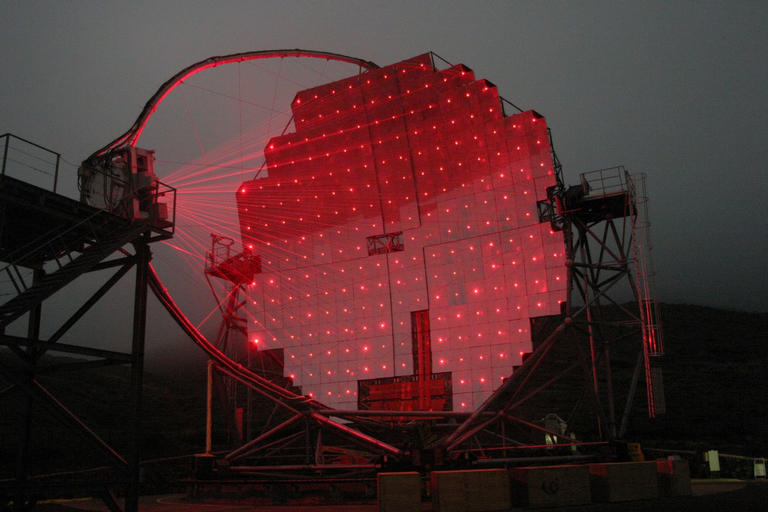
\includegraphics[width=0.4\linewidth]{MagicCalibration.jpg}}\\*
\vfill
%% CONTENT ENDS HERE

{
%%%%%%%%%%%%%%%%%%%%%%%%%%%%%%%%%%%%%%%%%%%%%%%%%%%%%%%%%%%%%%%%%%%%%%%%%%%%%%%%
%%%%%%%%%%%%%%%%%%%%%%%%%% DO NOT MODIFY THE TABLE BELOW %%%%%%%%%%%%%%%%%%%%%%%
%%%%%%%%%%%%%%%%%%%%%%%%%%%%%%%%%%%%%%%%%%%%%%%%%%%%%%%%%%%%%%%%%%%%%%%%%%%%%%%%
	\begin{tabular*}{16cm}{p{7.59cm} p{7.58cm}}
		\small Candidat-e:					&	\small Professeur-e(s) responsable(s):\\*[10pt]
		\small\textbf{\textsc{\Author}}		&	\small\textbf{\textsc{\Professor}}\\*[10pt]
		\footnotesize  Filière d’études : ISC	&	\footnotesize  \textbf{En collaboration avec:} UNIGE\\*[10pt]
		\footnotesize  {} & \footnotesize  Travail de bachelor soumis à une convention de stage en entreprise: \Convention\\*[20pt]
		\footnotesize  {} & \footnotesize  Travail soumis à un contrat de confidentialité: \Confidentiel\\*[10pt]
	\end{tabular*}\\*[1.9cm]
}
\end{center}
\end{spacing}

%\clearpage
\cleardoublepage
%%%%%%%%%%%%%%%%%%%%%%%%%%%%%%%%%%% LIST OF ACRONYMS  %%%%%%%%%%%%%%%%%%%%%%%%%%
% Acronym definitions
\newacronym{em}{EM}{Électromagnétique}
\newacronym{ctao}{CTAO}{Cherenkov Telescope Array Observatory}
\newacronym{iact}{IACT}{Imagin Athmospheric (or Air) Cherenkov Telescope}
\newacronym{esa}{ESA}{Euopean Space Agency}
\newacronym{le}{LE}{Low Energy}
\newacronym{he}{HE}{High Energy}
\newacronym{vhe}{VHE}{Very High Energy}
\newacronym{uhe}{UHE}{Ultra High Energy}
\newacronym{ehe}{EHE}{Extremely High Energy}
\newacronym{unige}{UNIGE}{Université de Genève}
\newacronym{infn}{INFN}{Istituto Nazionale di Fisica Nucleare}
\newacronym{leo}{LEO}{Low Earth Orbit}
\newacronym{sipm}{SiPM}{Silicon Photomultiplier}
\newacronym{nasa}{NASA}{National Aeronautics and Space Administration}
\newacronym{fpga}{FPGA}{Field Programmable Gate Arrays}
\newacronym{sst}{SST}{Small-Sized Telescope}
\newacronym{mst}{MST}{Medium-Sized Telescope}
\newacronym{lst}{LST}{Large-Sized Telescope}
\newacronym{asic}{ASIC}{Application Specific Integrated Circuits}
\newacronym{cnn}{CNN}{Convolutional Neural Network}
\newacronym{pe}{pe}{Photon-Électron}
\newacronym{hepia}{HEPIA}{Haute École du paysage, d'ingénierie et d'architecture de Genève}
\newacronym{cern}{CERN}{Conseil Européen pour la Recherche Nucléaire}

%\clearpage
\cleardoublepage
%%%%%%%%%%%%%%%%%%%%%%%%%%%%%%%%%%% LIST OF FIGURES %%%%%%%%%%%%%%%%%%%%%%%%%%%%
% !TeX spellcheck = fr_FR
\renewcommand{\listfigurename}{Liste des illustrations}
\listoffigures
\addcontentsline{toc}{chapter}{\listfigurename} % Adding toc entry

% \chapter*{Références des URL}
% \addcontentsline{toc}{chapter}{Réferences des URL} % Adding toc entry

% \printbibliography[keyword={urls}]
%\clearpage
\cleardoublepage
%%%%%%%%%%%%%%%%%%%%%%%%%%%%%%%%%%%% LIST OF TABLES %%%%%%%%%%%%%%%%%%%%%%%%%%%%
% !TeX spellcheck = fr_FR
\renewcommand{\listtablename}{Liste des tableaux}
\listoftables
\addcontentsline{toc}{chapter}{\listtablename} % Adding toc entry

\vspace*{14.4pt}

\vspace*{14.4pt}
\end{spacing}
%\clearpage
\cleardoublepage
%%%%%%%%%%%%%%%%%%%%%%%%%%%%%%%%%%% LIST OF ANNEXES %%%%%%%%%%%%%%%%%%%%%%%%%%%%
%%% COMMENT THIS PART IF YOU DO NOT USE DEDICATED TOC FOR ANNEXES AND COMMENT 
%%% HEADER AND FOOTER PART IN {chapters/annexes} FILE
% \begin{spacing}{1}
% % !TeX spellcheck = fr_FR
\chapter*{Liste des annexes} % No (numbered) toc entry with *
\addcontentsline{toc}{chapter}{Liste des annexes} % Adding toc entry

\printcontents[annexes]{ }{2}{}
% \end{spacing}
% %\clearpage
% \cleardoublepage
%%%%%%%%%%%%%%%%%%%%%%%%%%%%%%%%%%%%% INTRODUCTION  %%%%%%%%%%%%%%%%%%%%%%%%%%%%
\begin{spacing}{1.5}
\pagenumbering{arabic}
% !TeX spellcheck = fr_FR
\chapter*{Introduction}
\addcontentsline{toc}{chapter}{Introduction} % Adding toc entry

Dans le cadre de mon travail de bachelor, j'ai été choisi pour travailler avec le groupe "High-Energy Multi-Messenger" de l'\gls{unige}.
Ce groupe effectue des recherches expérimentales sur les particules provenant d'astres lointains à l'aide de satellites et de télescopes.
Leurs activités se concentrent majoritairement sur les rayons gamma, les rayons cosmiques et les neutrinos.
Mon travail consiste à aider cette équipe pour traiter des données concernant les rayons gamma et cosmiques à travers le phénomène physique de la radiation Cherenkov. 

Ce phénomène se produit lorsqu'une particule chargée se déplace à une vitesse supérieure à celle de la lumière dans un médium diélectrique transparent. 
L'exemple le plus notable de ce phénomène est la lumière bleutée produite dans l'eau autour d'un réacteur nucléaire. 
Cette lumière est due aux rayons gamma produits par la réaction nucléaire. Ces rayons, à cause des immenses forces électromagnétiques, se déplacent momentanément plus 
rapidement que la vitesse de la lumière dans l'eau.
On peut comparer ce phénomène à un boom supersonique mais pour de la lumière.

Les chercheurs de l'\gls{unige} s'intéressent cependant moins aux rayons gamma produits par des installations humaines qu'aux rayons et particules cosmiques provenant de l'espace.
Ces rayons et particules extraterrestres produisent aussi une radiation de Cherenkov mais dans le médium de notre atmosphère.
Lorsque le phénomène Cherenkov débute dans l'atmosphère, on appelle cela la "lumière Cherenkov".
Ce rayonnement va créer un cône de particules chargées qui sera détecté au sol à l'aide de télescopes. 

Aujourd'hui, ce phénomène est déjà étudié par de nombreux télescopes terrestres mais son observation est limitée par
divers bruits. Pour pallier à ceux-ci, il est prévu d'étudier ce phénomène depuis un télescope en orbite afin de les éviter au maximum.
Cependant, le satellite envisagé possède des limitations techniques, notamment sur la quantité d'informations qu'il peut envoyer ou recevoir.
Mon implication dans ce projet est de présenter un modèle de machine learning qui, en effectuant une étape de pré-traitement, aidera à cibler les
évènements détectés et, possiblement, à réduire la quantité de données à transmettre.

La première partie de ce rapport portera sur une explication du phénomène physique et de la façon dont il est détecté physiquement.
Une deuxième partie sera consacrée au déroulement du projet ainsi qu'aux intérêts scientifiques que celui-ci présente.
Une troisième partie expliquera de plus près les technologies et méthodes utilisées au cours de ce projet.
Le dernier chapitre présentera la réalisation du projet ainsi que les résultats obtenus suivi d'une conclusion.
%\clearpage
\cleardoublepage
%%%%%%%%%%%%%%%%%%%%%%%%%%%%%%%%%%%%%%% CHAPTERS %%%%%%%%%%%%%%%%%%%%%%%%%%%%%%%
%%%%%%%%%%%%%%%%%%%%%%%%%%%%%%% Add your chapters here %%%%%%%%%%%%%%%%%%%%%%%%%
%\input{chapters/chapXXX}
% !TeX spellcheck = fr_FR
\chapter{Chapitre 1 : Phénomène physique}

%TODO explain light in general ?

\section{La lumière Cherenkov}

L'effet Cherenkov a lieu lorsqu'une particule chargée électriquement traverse un milieu diélectrique transparent
en excédant la vitesse maximale de la lumière dans ce même milieu. 
Lors de son passage, cette particule va exciter les autres particules du milieu et produire une réaction en chaîne.
Cette dernière va donc créer un cône de particules tel que des électrons, positrons ou photons et même des particules élémentaires nommées hadrons.
Cet effet est similaire au bang supersonique lorsque des objets dépassent le mur du son mais dans le spectre électromagnétique.
Le cas le plus connu de cet effet est celui qui peut être observé autour des réacteurs nucléaires, dû à la lumière bleue qu'il engendre.

\begin{figure}[tbph!]
	\centering
	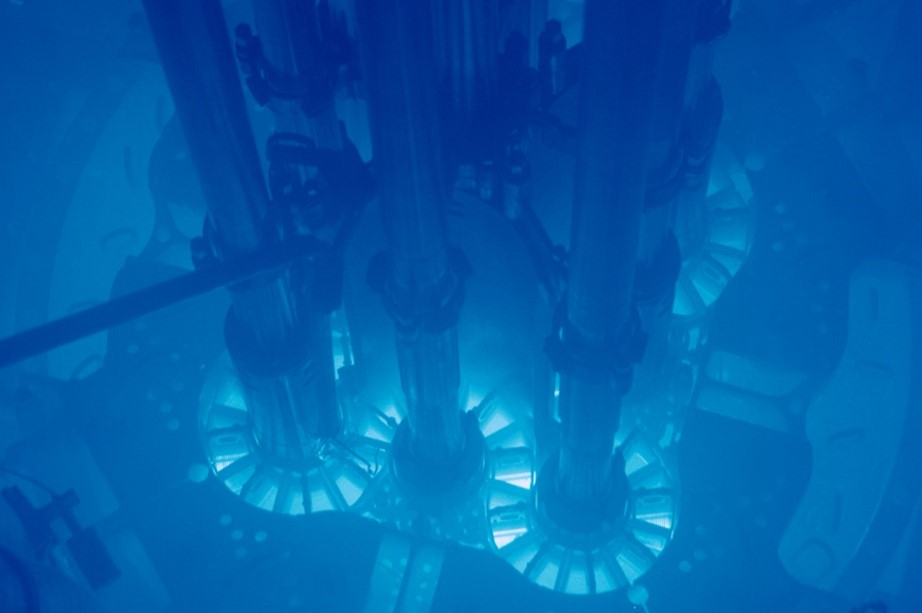
\includegraphics[width=0.6\linewidth]{cherenkov_radiation}
	\caption[Advanced Test Reactor core, Idaho National Laboratory]{Advanced Test Reactor core, Idaho National Laboratory. Source : \cite{CherenkovRadiation}}
\end{figure}

%TODO better redaction ?
L'intensité de la lumière est communément quantifiée en électron-volt ou eV.
Cette unité représente l'énergie cinétique gagnée lorsqu'un électron voit son énergie potentielle augmentée d'un Volt dans le vide.
%END TODO

La lumière Cherenkov atmosphérique peut produire deux types de pluies différentes : les pluies purement \gls{em}
composées uniquement d'électrons, positrons et photons ainsi que les pluies hadroniques qui elles sont composées de hadrons chargés électriquement, comme des protons.

\begin{figure}[tbph!]
	\centering
	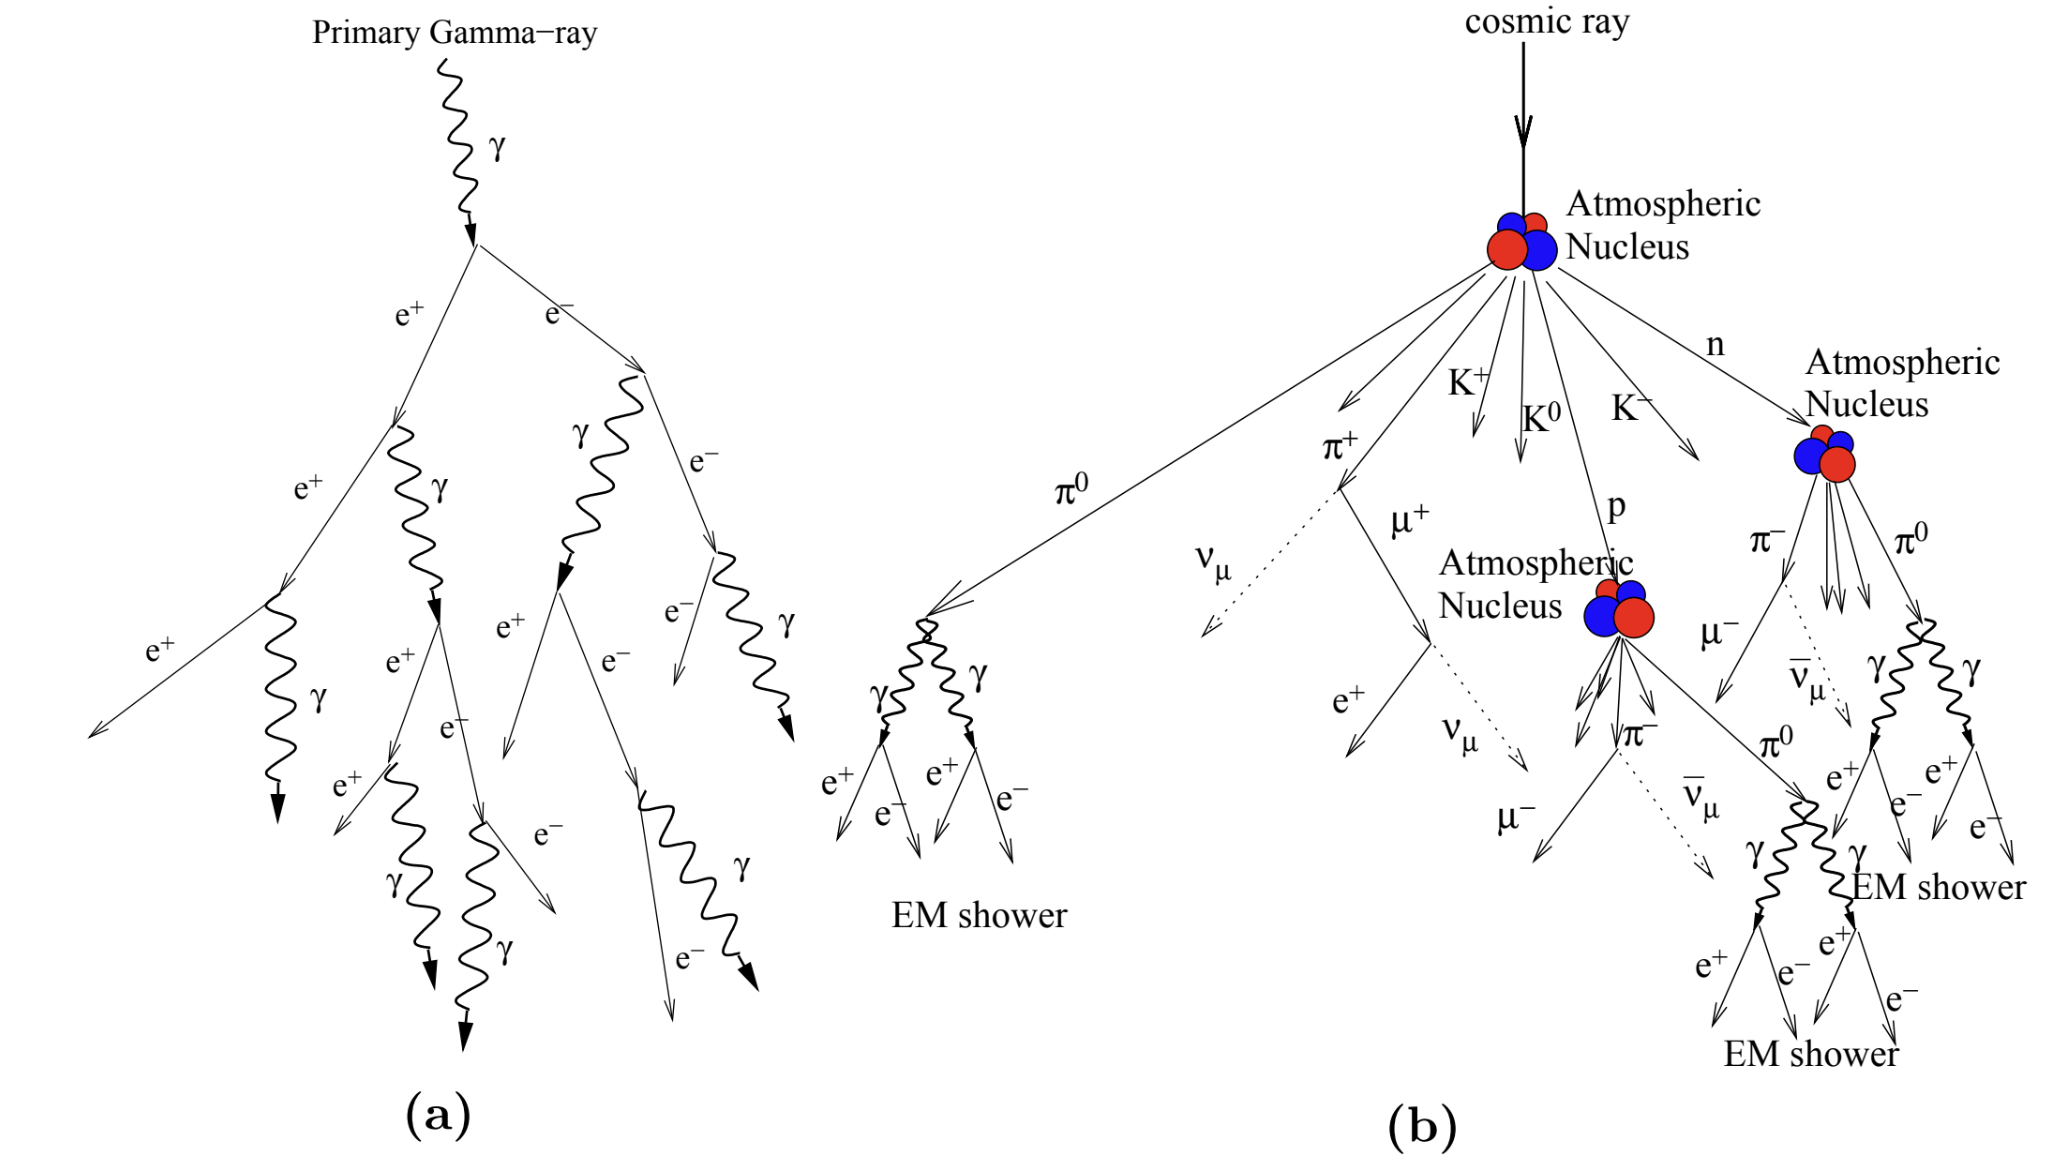
\includegraphics[width=\textwidth]{cherenkov_showers.png}
	\caption[Diagramme de pluies EM et hadroniques]{Diagramme de pluies électromagnétiques pures (a) et pluies hadroniques (b). Source : I. Oya Vallejo. “Observation of active galactic nuclei with the Magic telescope”. UCM. PhD thesis. 2010.}
\end{figure}

Les pluies hadroniques sont généralement plus puissantes que des pluies \gls{em} et ont voit aussi qu'elles se décomposent au fur et à mesure en pluies \gls{em}.
Pour les pluies \gls{em}, la production d'électrons et de positrons se fait via deux principes physiques : la production de paires et par rayonnement continu de freinage.
La production de paires se produit lorsqu'une particule chargée à haute énergie interagit aux abords du noyau d'une autre particule.
Suite à cette interaction un électron et un positron sont produits. Ces deux particules vont ensuite créer à leur tour des photons 
lorsqu'elles ralentissent autour d'autres noyaux. Ce ralentissement a comme conséquence de produire un photon.

\begin{figure}[!tbp]
	\centering
	\begin{minipage}[b]{0.4\textwidth}
	  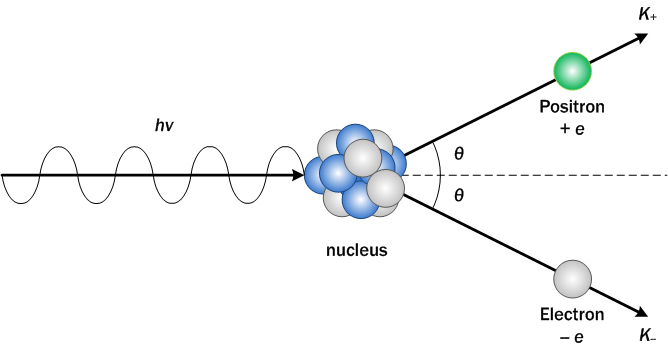
\includegraphics[width=\textwidth]{PairProduction.jpg}
	  \caption[Création de paires]{Diagramme de création de paires. Source : \cite{PairProduction}}
	\end{minipage}
	\hfill
	\begin{minipage}[b]{0.4\textwidth}
	  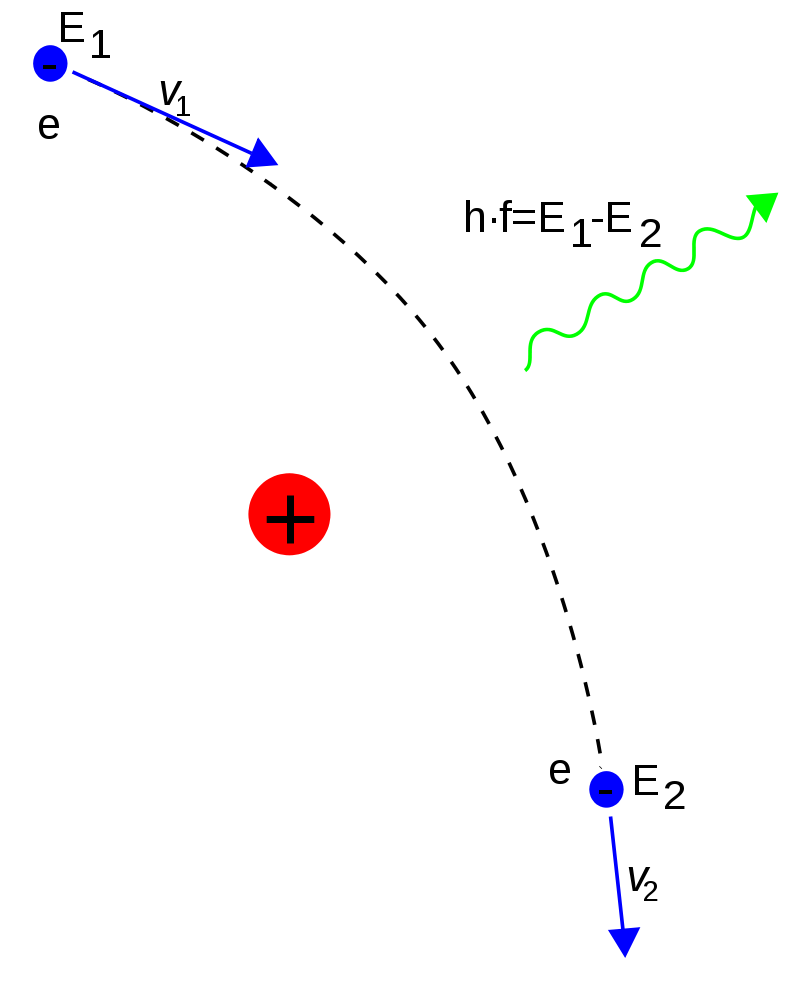
\includegraphics[width=\textwidth]{RayonnementContinuDeFreinage.png}
	  \caption[Rayonnement continu de freinage]{Diagramme de rayonnement continu de freinage. Source : \cite{Bremsstrahlung}}
	\end{minipage}
\end{figure}

L'intérêt scientifique se porte cependant plus sur les pluies \gls{em} pures à cause des rayons gamma qui débutent la réaction en chaîne.
Comparés aux particules chargées comme des protons, les rayons gamma eux ne sont pas déviés par les champs électriques ou magnétiques 
pendant leur trajet à travers les astres. En détectant ces pluies purement \gls{em}, on peut en déduire leur provenance beaucoup plus simplement 
que pour des pluies hadroniques où il faut prendre en compte les différentes interactions astronomiques et atmosphériques.

% TODO energy levels for gamma / hadronic split

\section{Méthodes de détection}
Les rayons gamma varient grandement en intensité de quelques MeV jusqu'à des dizaines de PeV et plus encore jusqu'au maximum ~100 EeV. \cite{TjarkPHD}
En fonction de l'énergie d'un rayon gamma, certaines techniques sont plus optimisées que d'autres, ici on retrouve les différentes techniques utilisées aujourd'hui :

% TODO Better explanation of physics for actual detection
% Chaque tube photomultiplicateur est capable de quantifier l'énergie reçue par des photons en entrée du capteur et il "stocke" cette valeur en tant que charge électrique. 
% En échantillonnant cette charge électrique a intervalle réguliers on retrouve une forme d'onde de l'amplitude détectée sur le temps.
%END TODO
\begin{table}[tbph!]
	\centering{
		\begin{tabular}{ |c|c|c|c| }
			\hline
			\textbf{Notation} & \textbf{Gamme d'énergie} & \textbf{Technique de détection} & \textbf{Emplacement} \\
			\hline
			LE & < 30 MeV & Photoélectrique, Compton & Espace \\
			\hline
			HE & 30 MeV à 100 TeV & Création de paires & Espace \\
			\hline
			VHE & 100 GeV à 30 TeV & Cherenkov (atmosphérique) & Terrestre \\
			\hline 
			UHE & 30 TeV à 30 PeV & Cherenkov (eau) & Terrestre \\
			\hline 
			EHE & > 30 PeV & Fluorescence, Hybride & Terrestre \\
			\hline 
		\end{tabular}
		\caption[Techniques de détection en fonction de la classification énergétique des rayons gamma]{Techniques de détection en fonction de la classification énergétique des rayons gamma. Source : \cite{TjarkPHD} p. 17}
	}
\end{table}

\section{Astronomie gamma existante}
\subsection{INTEGRAL}
En l'an 2002, l'\gls{esa} a lancé le satellite INTEGRAL qui est le premier à avoir observé les spectres \gls{em} visible, x-ray et gamma en simultané.
Concernant les rayons gamma, ce satellite est équipé de deux capteurs englobant la plage de rayons gamma \gls{le} de ~15keV à ~10MeV \cite{IntegralSpecs} 

\begin{figure}[tbph!]
	\centering
	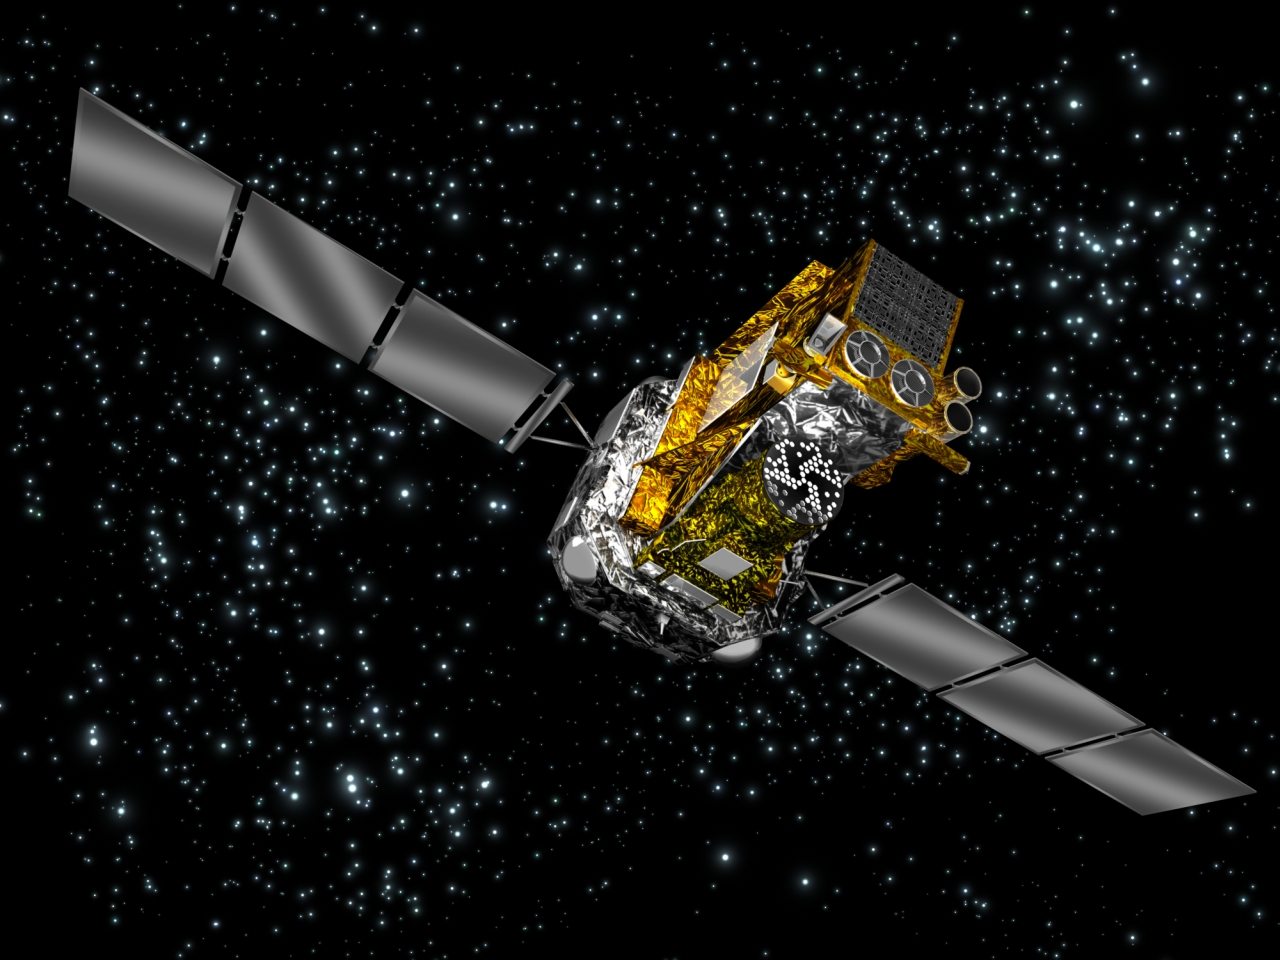
\includegraphics[width=0.4\linewidth]{Integral}
	\caption[Illustration du satellite INTEGRAL]{Illustration du satellite INTEGRAL. Source : \cite{IntegralImage}}
\end{figure}

\subsection{Fermi-LAT}
Le satellite Fermi a été développé par la \gls{nasa} en collaboration avec des institutions
françaises, allemandes, japonaises, italiennes et suédoises. Il a été envoyé en orbite en 2008 et il est en opération depuis lors. \cite{Fermi}
Il transporte deux instruments de mesures : le Large Area Telescope (20 MeV à > 300 GeV) et le Gamma-ray Burst Monitor (8 keV à 40 MeV).

Le détecteur fonctionne via la détection de production par paires à l'intérieur du détecteur après une collision d'un photon.
Les trajectoires et l'énergie dégagée par cet impact ressemble aux expériences des accélérateurs de particules.

L'observatoire fonctionne normalement en un mode de découverte qui scanne tout le spectre gamma du ciel.
Il est capable de scanner l'entièreté du ciel en seulement deux orbites.
Il a par exemple découvert les bulles de Fermi qui sont d'immenses sources de rayons gamma dans notre Voie lactée. 
Celles-ci proviendraient de grandes décharges d'énergie émises par le trou noir central de la galaxie il y a de cela plusieurs millions d'années.

\begin{figure}[tbph!]
	\centering
	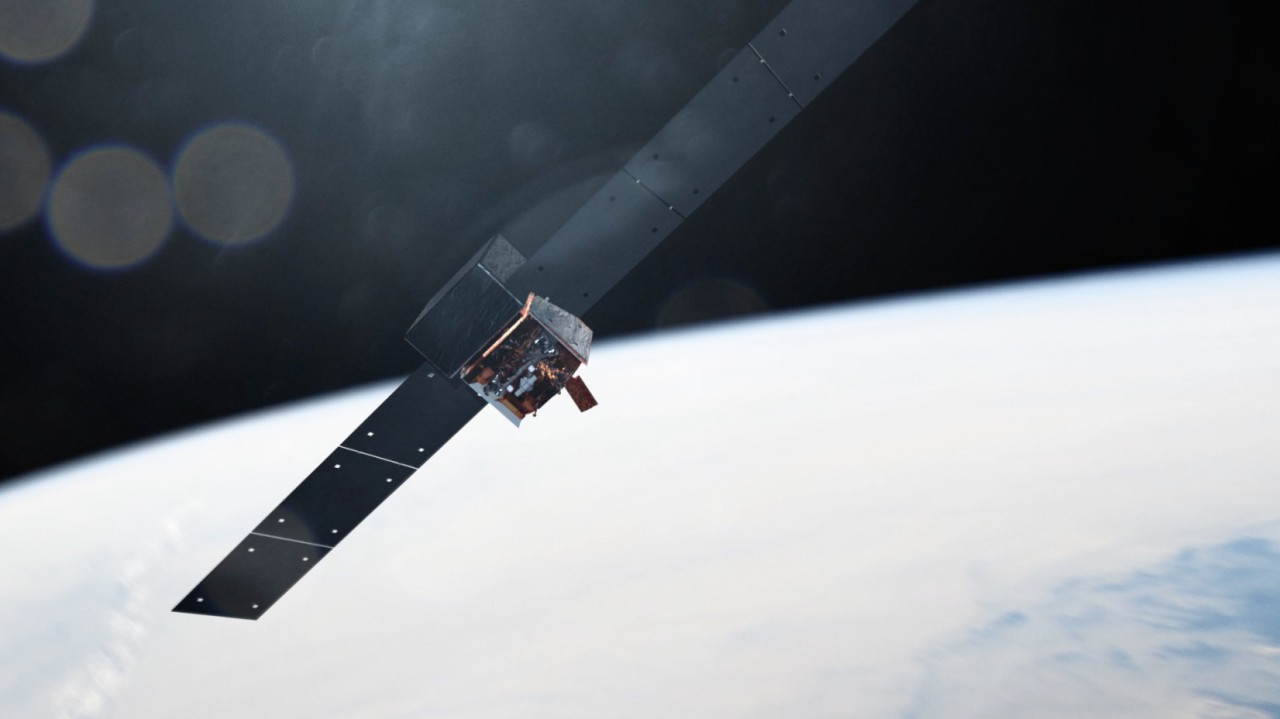
\includegraphics[width=0.5\linewidth]{fermi.jpg}
	\caption[Illustration du Fermi Gamma-ray Space Telescope en orbite]{Illustration du Fermi Gamma-ray Space Telescope en orbite. Source : \cite{FermiImage}}
\end{figure}

\subsection{MAGIC}
\textbf{MAGIC} est une installation de deux télescopes \gls{iact} complétée en 2009 à l'observatoire "Observatorio del Roque de los Muchachos" situé à La Palma aux îles
Canaries a une altitude d'environ 2200m. \cite{Magic}

Les télescopes ont été conçus pour étudier les rayons gamma \gls{vhe} de 30GeV à 100 TeV grace à leurs miroirs de 17m de diamètre qui réfléchissent la lumière dans
une grille hexagonale de 1039 tubes photomultiplicateurs, ce qui leur permet de visualiser le ciel avec un champ de vision du ciel de 3,5°.

\begin{figure}[tbph!]
	\centering
	\includegraphics[width=0.6\linewidth]{MAGIC.jpg}
	\caption[Photo des deux télescopes MAGIC]{Photo des deux télescopes MAGIC. Source : \cite{MagicImage}}
\end{figure}

\subsection{H.E.S.S.}
Le \textbf{High Energy Stereoscopic System} était initialement une installation de 4 télescopes de 12m formant un carré de 120m de côté rendu opérationnel en 2004 dans la région de Khomas en Namibie.
En 2012, un 5ème télescope de 28m et 580 tonnes a été ajouté au centre de ce carré, augmentant la sensibilité en la résolution angulaire du système. \cite{Hess}

Les quatre télescopes aux extrémités ont un champ de vision de 5° et sont équipés de caméras composées de 960 tubes photomultiplicateurs.
Le télescope central possède aussi une caméra composée de 2048 photomultiplicateurs avec un champ de vision de 3,2°.

\begin{figure}[tbph!]
	\centering
	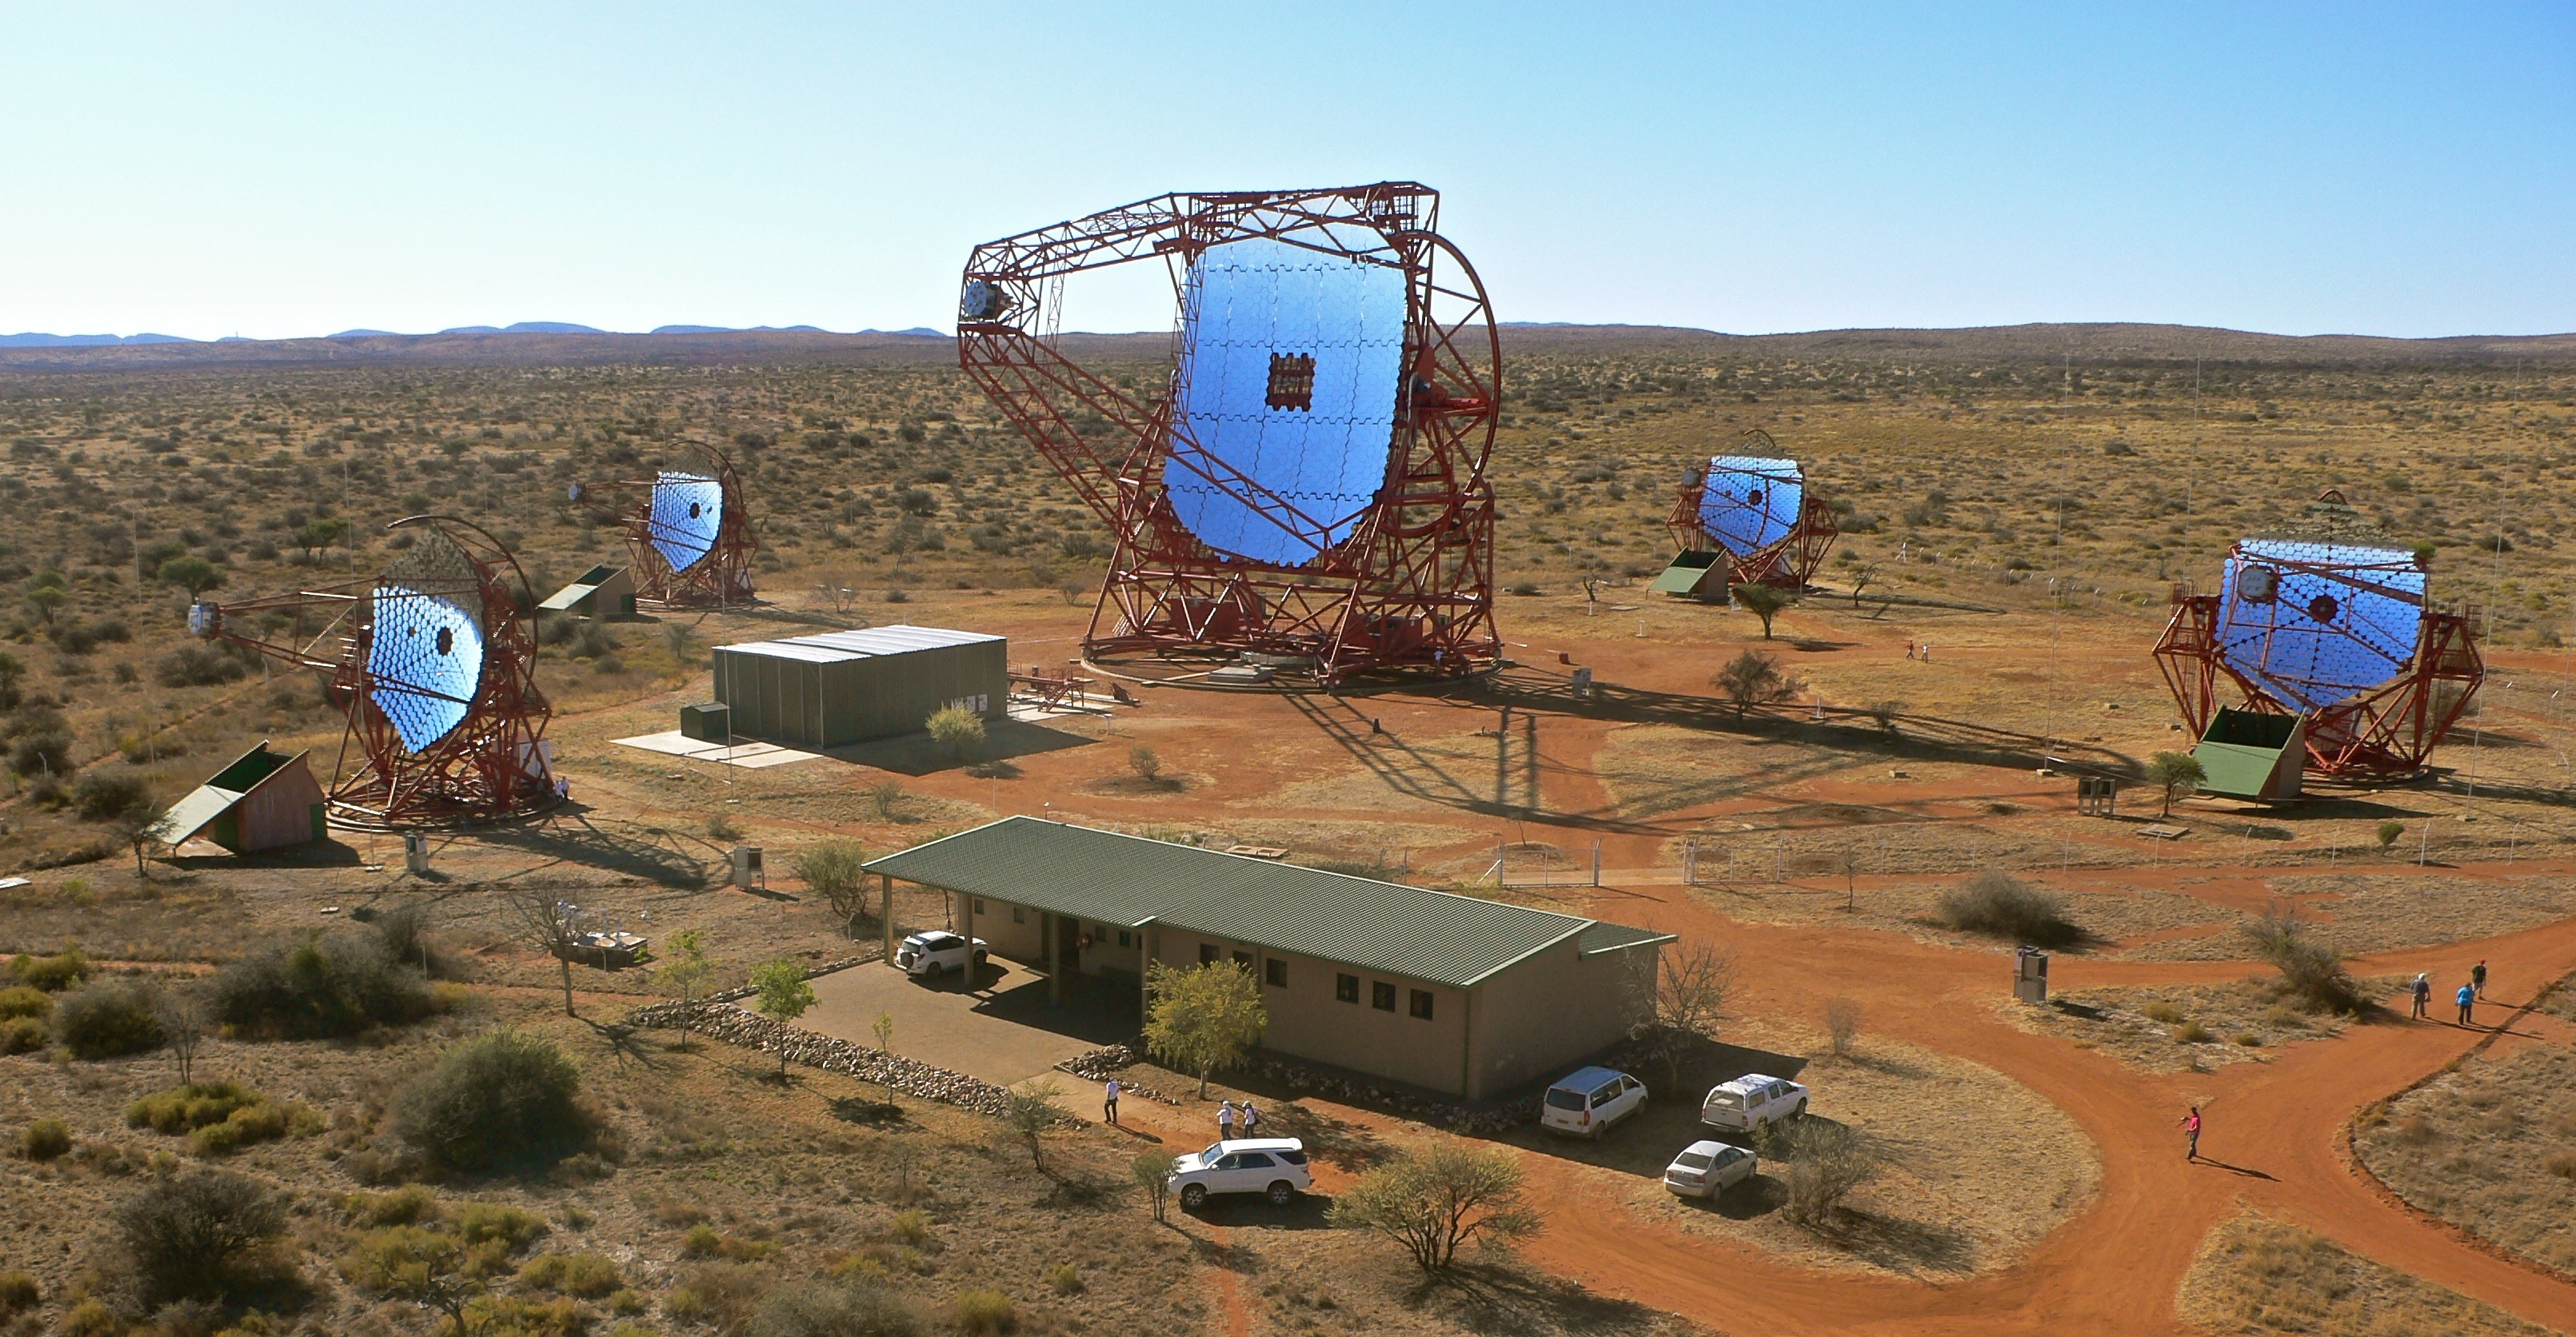
\includegraphics[width=0.6\linewidth]{hess.jpg}
	\caption[Photo de l'installation H.E.S.S]{Photo de l'installation H.E.S.S. Source : \cite{HessImage}}
\end{figure}

\subsection{VERITAS}
Le \textbf{Very Energetic Radiation Imaging Telescope Array System} est un projet financé par les USA, le Canada et l'Allemagne installé au Fred Lawrence Whipple Observatory dans l'Arizona.
Il est composé de quatre télescopes de 12m d'ouverture avec des caméras chacune composées de 499 tubes photomultiplicateurs. \cite{Veritas} 
L'installation a pour but d'étudier les rayons gamma \gls{vhe} entre 50GeV et 50TeV et a notamment été utilisée pour complémenter la mission Fermi de la \gls{nasa}.

\begin{figure}[tbph!]
	\centering
	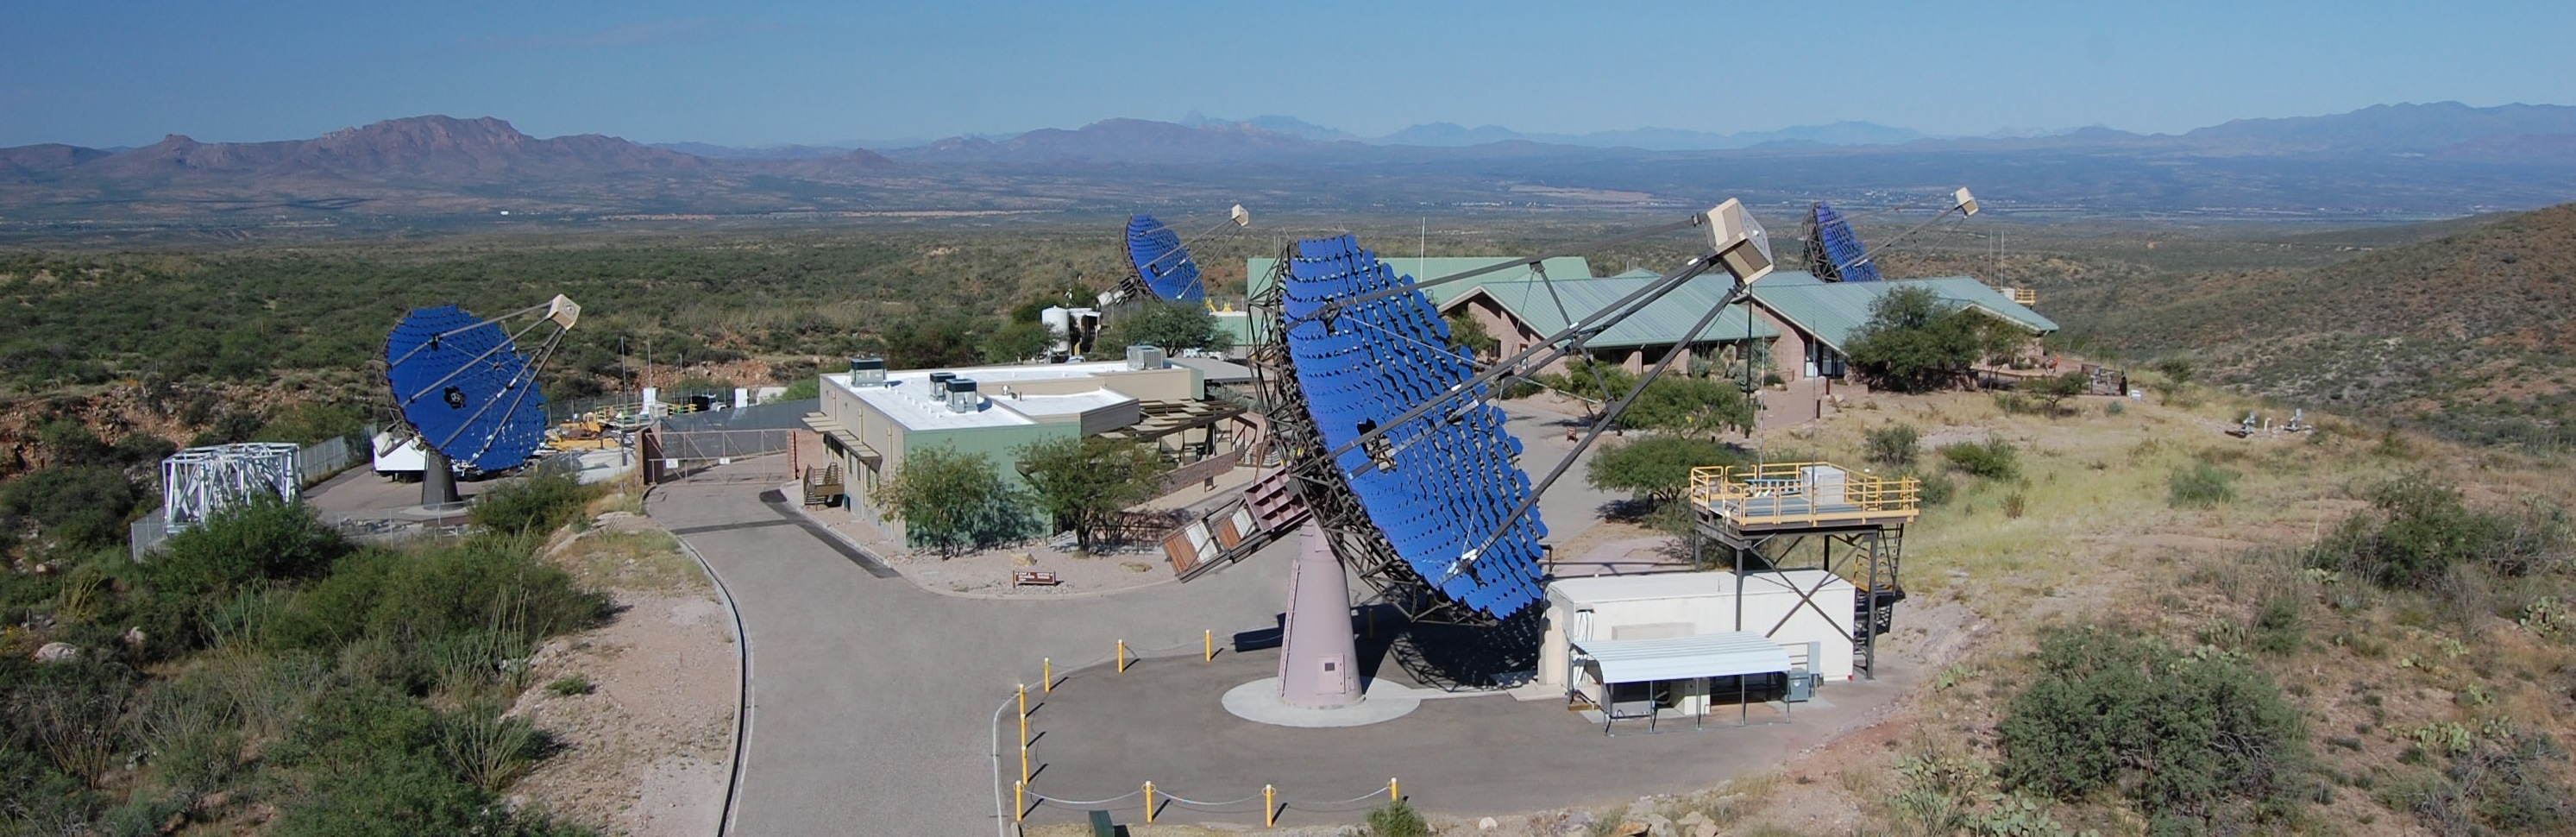
\includegraphics[width=0.8\linewidth]{veritas.jpg}
	\caption[Fred Lawrence Whipple Observatory]{Fred Lawrence Whipple Observatory. Source : \cite{Veritas}}
\end{figure}

\subsection{HAWC}
HAWC pour \textbf{High altitude Water Cherenkov gamma-ray observatory} est un observatoire situé sur le flanc du volcan Sierra Negra au Mexique, à une altitude de 4100 mètres.
Comme son nom l'indique, il observe la lumière Cherenkov dans de l'eau au lieu de l'atmosphère. Ceci permet d'étudier des rayons gamma de plus haute intensité, de 100GeV à 100TeV. \cite{Hawc}

Au lieu d'utiliser des photomultiplicateurs comme les télescopes précédents, HAWC utilise des compteurs de particules basés sur des scintillateurs.
% TODO refaire phrase
Cette différence de fonctionnement comparé aux \gls{iact} lui permet de meilleures performances dans certains domaines tel le champ de vision mais le rend plus sensible au bruit de fond par exemple :

\begin{table}[tbph!]
	\centering{
		\begin{tabular}{ |c|c|c| }
			\hline
			 & \textbf{Télescope Cherenkov} & \textbf{Détecteur de Pluie Atmosphérique} \\
			\hline
			\textbf{Gamme d'énergie} & Basse (<200 GeV) & Haute (>10TeV) \\
			\hline
			\textbf{Rejet de bruit de fond} & Excellent (>99.7\%) & Modéré (>50\%) \\
			\hline
			\textbf{Champ de vision} & Petit (<2°) & Large (>45°) \\
			\hline 
			\textbf{Disponibilité} & Basse (5\%-10\%) & Haute (>90\%) \\
			\hline
		\end{tabular}
		\caption[Complementary detection characteristics of imaging air Cherenkov telescopes (IACTs) and extensive air shower arrays.]{Complementary detection characteristics of imaging air Cherenkov telescopes (IACTs) and extensive air shower arrays, traduit. Source : \cite{Hawc}}
	}
\end{table}

\begin{figure}[tbph!]
	\centering
	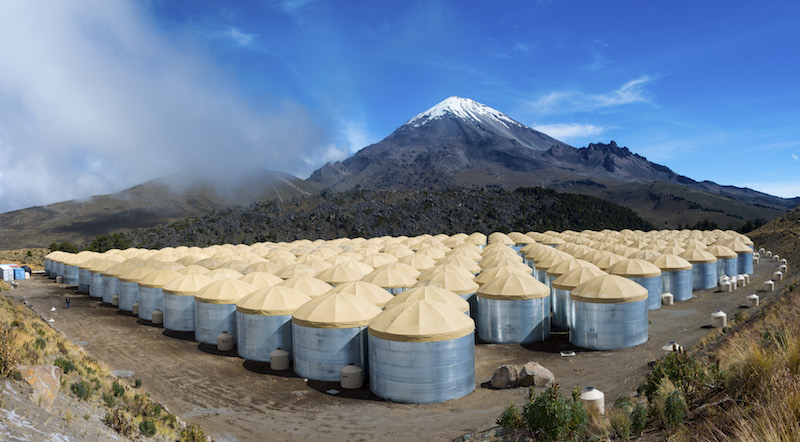
\includegraphics[width=0.6\linewidth]{hawc.jpg}
	\caption[The HAWC Observatory]{The HAWC Observatory. Source : J. Goodman, Nov. 2016 \cite{Hawc}}
\end{figure}

\section{Astronomie gamma future}
\subsection{CTAO}
Le \gls{ctao} est le plus grand projet d'observatoire \gls{iact} au monde. Il est prévu de construire 60 télescopes répartis sur 2 sites, 
le premier (CTAO-North) dans l'hémisphère nord aux îles Canaries sur l'île La Palma et le deuxième (CTAO-South) à Paranal, Chili.

% \begin{figure}[tbph!]
% 	\centering
% 	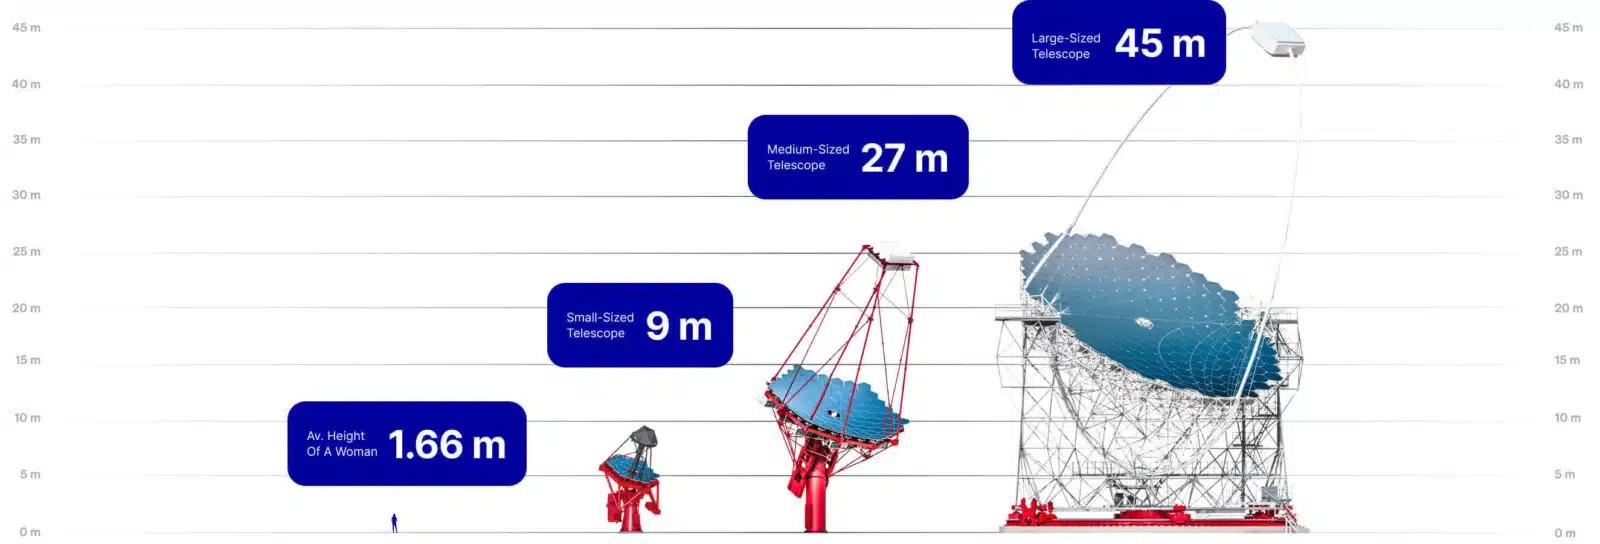
\includegraphics[width=0.8\linewidth]{ctao_telescopes.jpg}
% 	\caption[Illustration des différents télescopes du CTAO]{Illustration des différents télescopes du CTAO. Source : CTAO \cite{Ctao}}
% \end{figure}

L'observatoire est conçu pour étudier les rayons gamma de 20GeV à 300TeV avec plus de 60 télescopes de différentes tailles, \gls{sst}, \gls{mst} et \gls{lst} qui peut atteindre 45m de haut
Pour cela chacun des types de télescopes a été conçu pour répondre au mieux à certaines gammes d'énergie.
Pour la gamme principale de l'installation (150GeV à 5TeV), ce sont 23 \gls{mst} qui sont prévu d'être construire.
37 \gls{sst} sont prévus et ils seront optimisés pour détecter les énergies > 5TeV et jusqu'à 4 \gls{lst} sont prévus pour détecter les gammes d'énergie < 150 GeV.

\begin{figure}[tbph!]
	\centering
	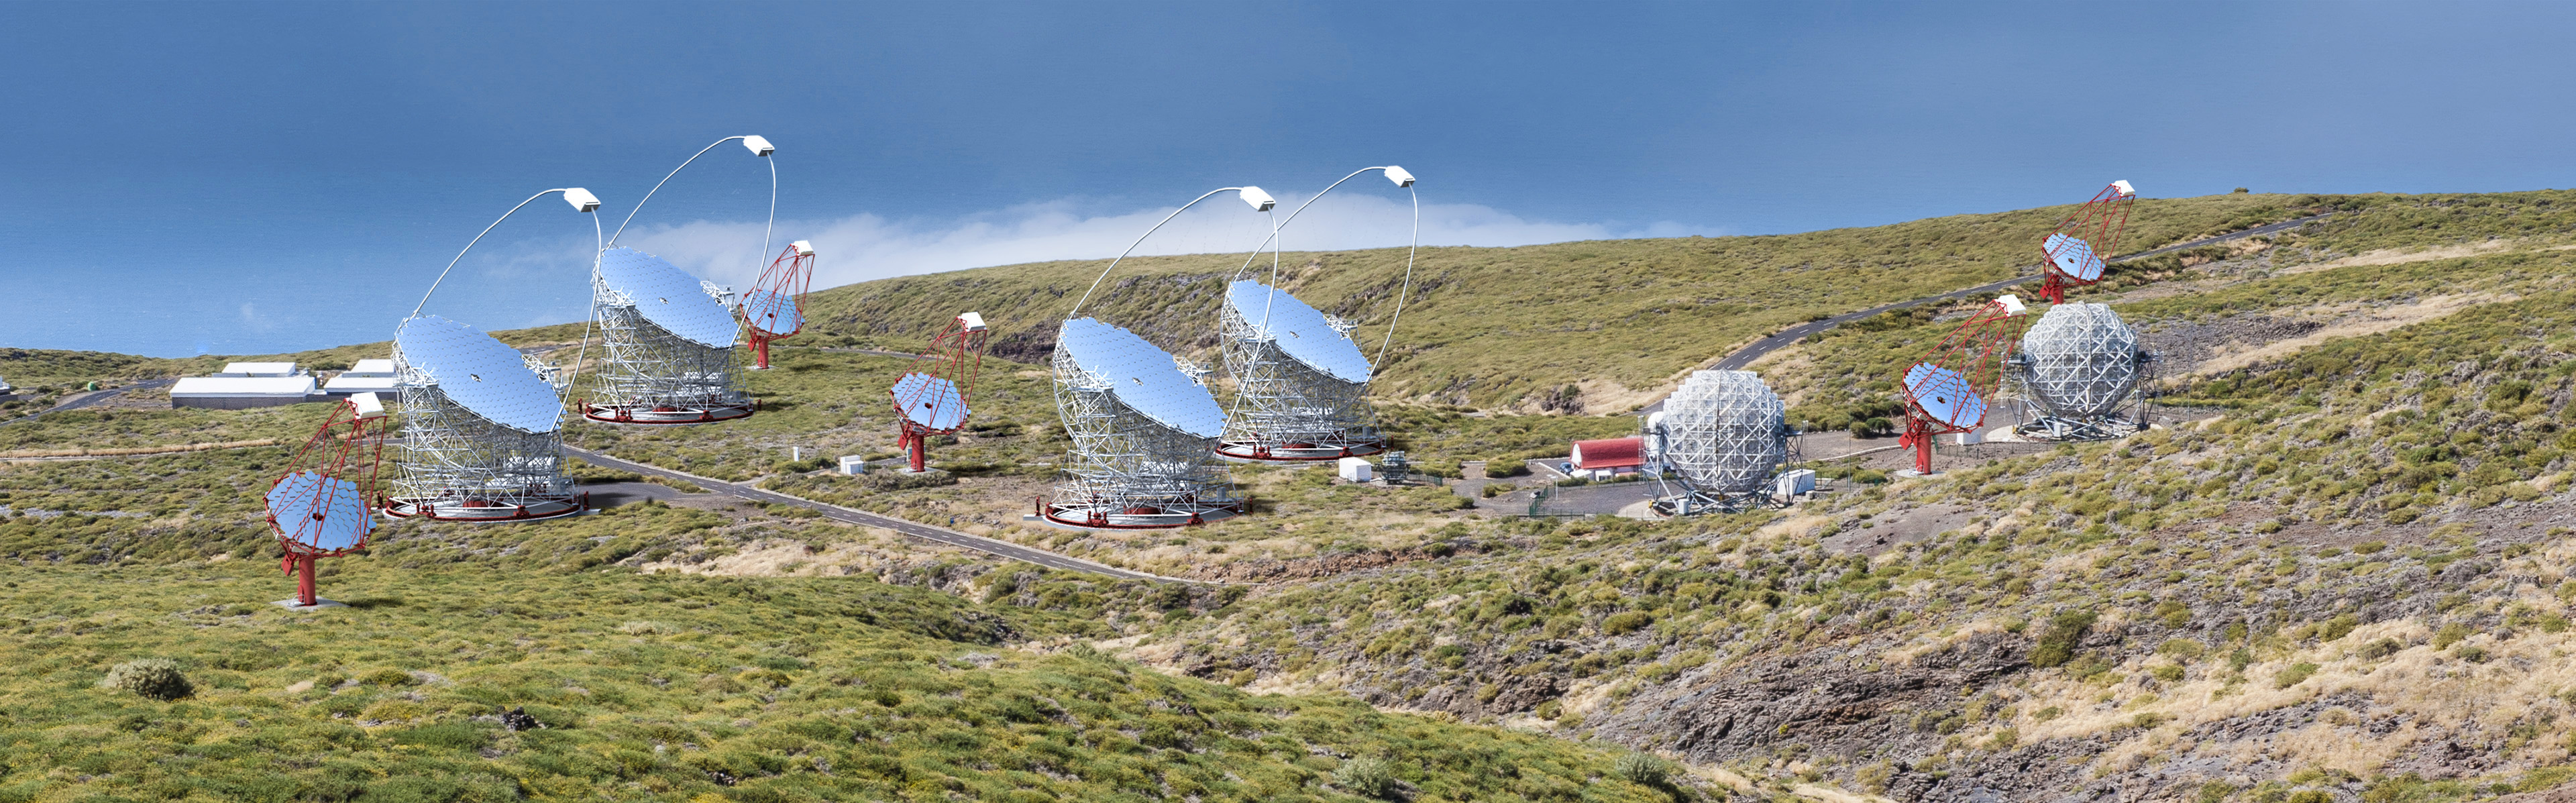
\includegraphics[width=0.9\linewidth]{ctao.jpg}
	\caption[Rendu 3d de CTAO-North]{Rendu 3d de CTAO-North. Source : Gabriel Pérez Díaz, IAC \cite{CtaoImage}}
\end{figure}


% \subsection{ASTRI}
% !TeX spellcheck = fr_FR
\chapter{Chapitre 2 : Historique du projet}

\section{Projet initial}

En novembre 2023, l'\gls{unige} a contacté l'\gls{hepia} afin de créer un projet commun sur la recherche d'un modèle de 
réseau neuronal à très basse consommation et embarquable pour le projet du télescope spatial Terzina. 
Le but de ce modèle serait d'aider à la décision d'événements scientifiquement intéressants 
détectés par le télescope afin de réduire la quantité d'informations à transmettre au sol. 
Il est prévu d'envoyer le télescope Terzina à bord du satellite NUSES.

\subsection{NUSES}
Le projet \textbf{NeUtrino and Seismic Electromagnetic Signals} est une mission spatiale pionnière qui 
a vu le jour via la collaboration entre différentes universités et organisations gouvernementales. \cite{Nuses}
Notamment l'\gls{unige}, l'\gls{infn} et la NASA.
Son but est d'envoyer un satellite dans l'espace avec deux instruments scientifiques à bord, Zirè et Terzina, qui mènerons 
des expériences une fois en orbite.

\begin{figure}[tbph!]
	\centering
	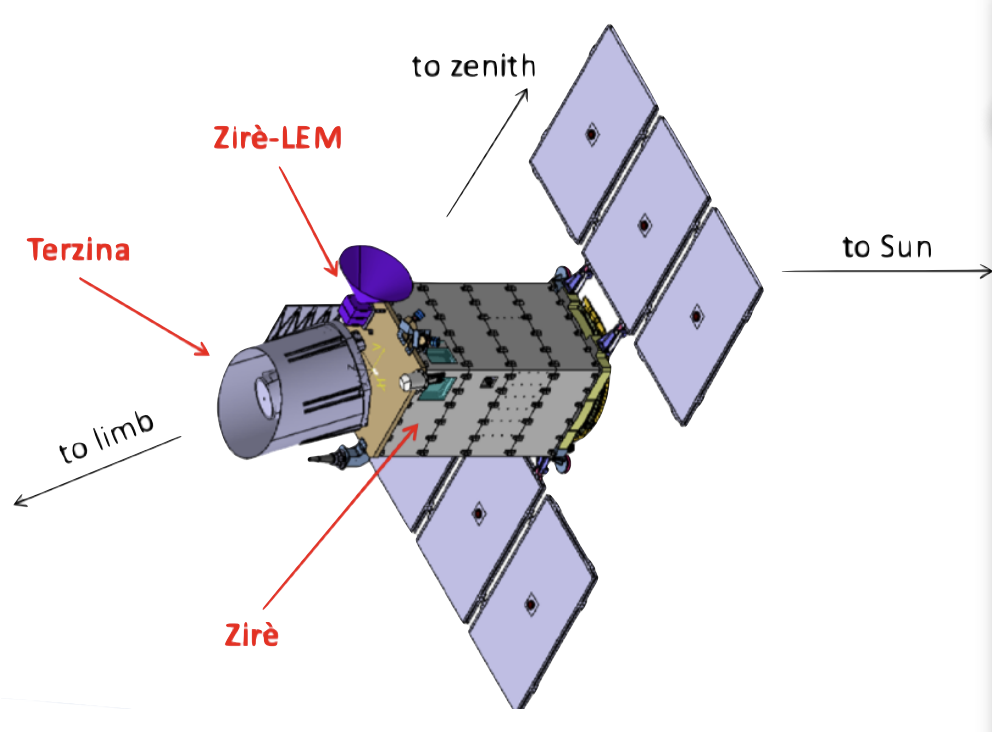
\includegraphics[width=0.7\linewidth]{nuses.png}
	\caption[Mission NUSES]{Mission NUSES. Source: \cite{Nuses}}
\end{figure}

\textbf{Zirè} a pour but d'observer le rayonnement cosmique \gls{le} (<250 MeV) pour étudier de plus près la ceinture de Van Allen,
la météo spatiale et les interactions entre les lithosphère, ionosphère et magnétosphère.

\textbf{Terzina} a pour but de tester de manière concrète les technologies qui pourraient être utilisées pour étudier des rayonnements cosmiques
\gls{uhe} > 100 PeV et de détecter des neutrinos via les pluies atmosphériques de lumière Cherenkov qu'ils produisent.

%comparaison with the Japanese detector in mountains ?

Le satellite sera placé en orbite terrestre basse de manière héliosynchrone.
L'orbite terrestre basse ou \gls{leo} est définie comme toutes les orbites plus proches que 1000 km au dessus de la surface de la terre.\cite{LowEarthOrbit}
L'orbite héliosynchrone est une orbite presque polaire (naviguant du nord au sud ou inversement) où le satellite 
passe au dessus d'un même point à la même heure solaire. Cela implique que son orientation en rapport au soleil reste la même.

Pour Terzina, cela permet aux capteurs d'être toujours pointés en direction opposée au soleil pour éviter au maximum les rayons gamma qu'il émet.

\begin{figure}[tbph!]
	\centering
	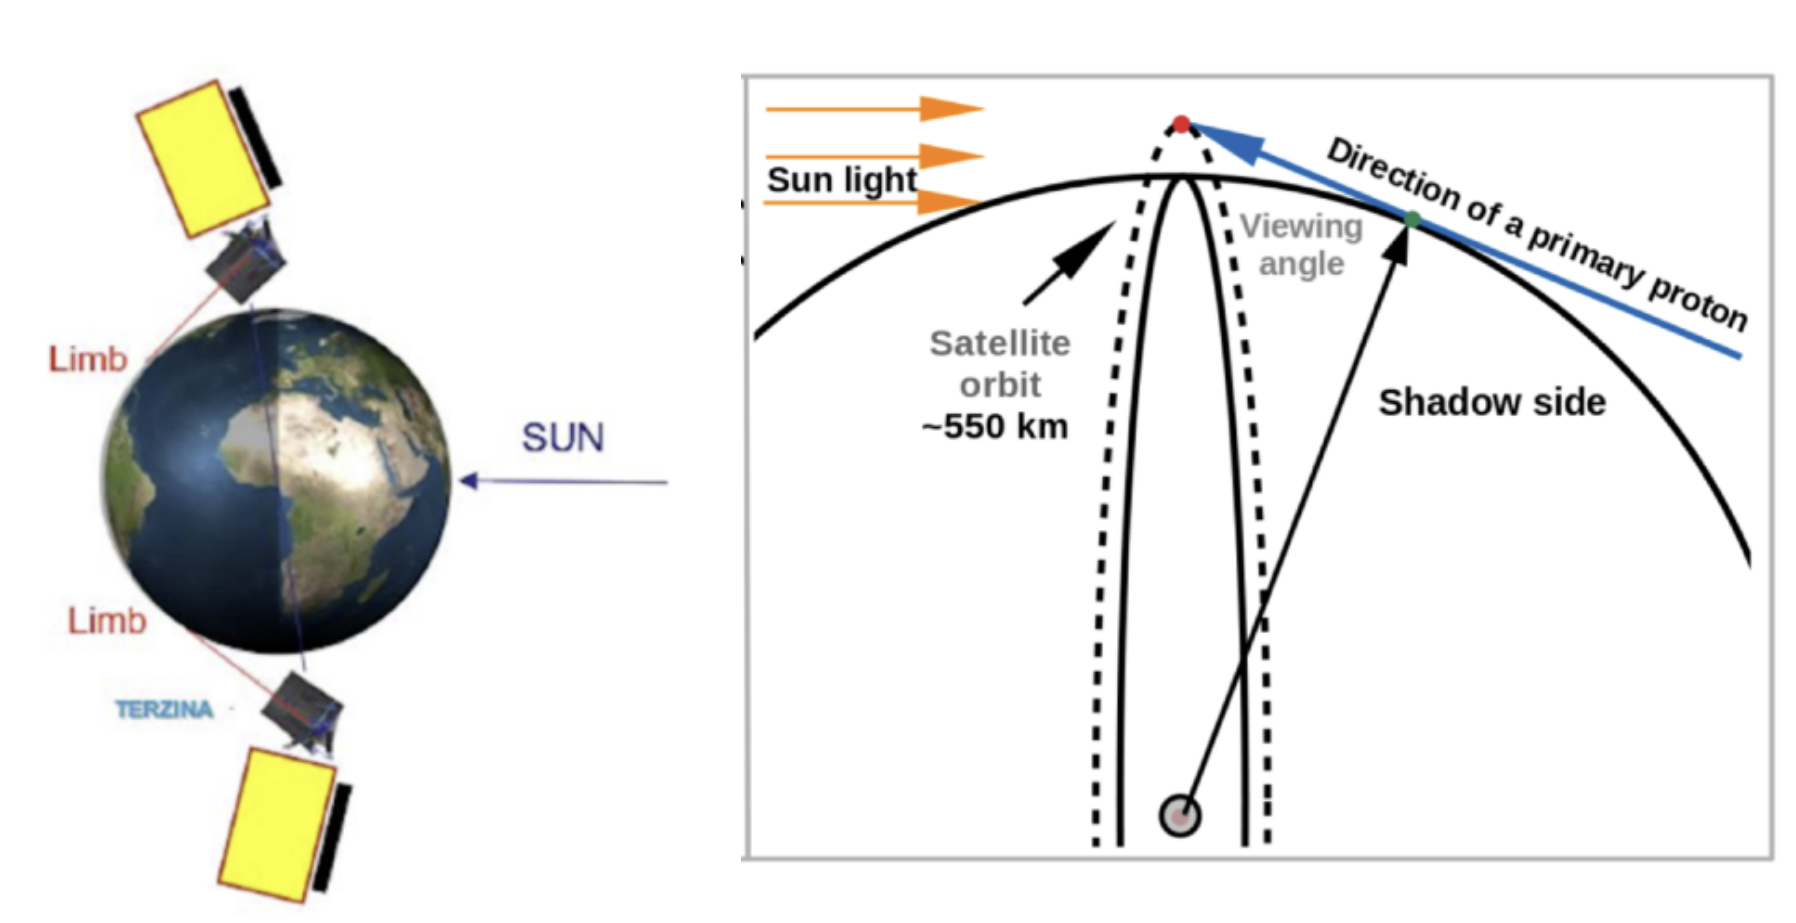
\includegraphics[width=0.7\linewidth]{heliosynchrone.png}
	\caption[Orbite héliosynchrone de Terzina]{Orbite héliosynchrone de Terzina. Source: \cite{Nuses}}
\end{figure}

\subsection{Terzina}
Comparé aux autres satellites qui ont étudiés des rayons gamma en orbite, Terzina est prévu d'être le premier télescope spatial
qui détectera la lumière Cherenkov depuis l'espace. De plus, il permettra aussi d'étudier les performances de nouveaux capteurs \gls{sipm}
dans l'espace. Ceux-ci devraient détecter plus de photons et être plus robustes que leur contrepartie classique bien que ces nouveaux capteurs
soient plus sensibles aux bruits de fond et à l'irradiation abondante hors de notre atmosphère.

\begin{figure}[tbph!]
	\centering
	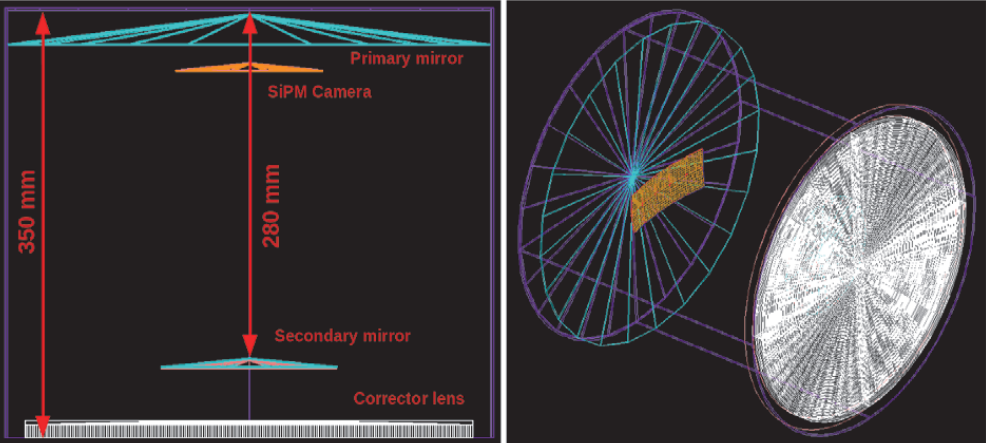
\includegraphics[width=0.7\linewidth]{terzina_mirrors.png}
	\caption[Vue de la configuration optique de Terzina]
	{En bleu les miroirs, en blanc la lentille, en orange la caméra et en violet les murs \textbf{Gauche :} Vue de dessus. \textbf{Droite :} Vue de côté. Source: \cite{Burmistrov_2023} p.2}
\end{figure}

Le télescope utilise une configuration à deux miroirs qui redirigent et concentrent les photons reçus sur une matrice 
rectangulaire de 10 modules \gls{sipm}, eux-mêmes possédant une résolution de 8x8 pixels, 640 pixels au total. \cite{Burmistrov_2023}

Cette forme rectangulaire a été décidée pour observer le limbe terrestre de manière optimale et elle est capable de détecter une coupe transversale de 140 x 360 $km^2$.
Derrière les 10 modules \gls{sipm}, il est prévu 10 \gls{asic} chacun possédant 64 canaux pour chacun des tubes photomultiplicateurs de la caméra.
Ces \gls{asic} sont conçus pour amplifier le signal de sortie puis le numériser avant d'être collectés par un \gls{fpga} à bord du satellite. 

En plus de leur rôle de numérisation, les \gls{asic} ont aussi le rôle de déclencheur matériel. 
Ce rôle est important pour que le signal analogue des photomultiplicateurs ne soit converti en signal numérique que si nécessaire. 

Le premier mécanisme de déclenchement, nommé "haut", arrive lorsqu'un pic d'énergie dépasse un seuil "haut" dans un seul canal
d'un module \gls{sipm}; chaque canal du module est numérisé et collecté par le \gls{fpga}. 

Le deuxième mécanisme de déclenchement "bas" arrive lorsque deux pixels adjacents d'un même module \gls{sipm}
dépassent ce seuil ou lorsque c'est l'un des 8 pixels voisins d'un autre module. 
Ensuite, les pixels voisins sont analysés pour déterminer si au moins deux d'entre eux ont aussi dépassé ce seuil "bas"; dans ce cas l'\gls{fpga} va conserver cet évènement.
Tous ces tests se déroulent dans un laps de temps très court; de la numérisation du signal aux traitement et stockage sur le \gls{fpga}, il se passerait environ 51.2$\mu$s

\section{Proposition de projet par l'UNIGE}

La quantité de données récoltées par Terzina se révèle être trop importante pour être envoyée au sol, même après l'activation des déclencheurs intégrés au matériel.
En effet, la capacité de bande passante de Terzina est limitée à 40Gbit par jour en transmission et seulement quelques Kbit par jour en réception.
Ceci est dû à la configuration du satellite NUSES qui est aussi partagé entre les deux instruments Zirè et Terzina.

C'est au moment de la conception que l'UNIGE a eu l'idée d'ajouter un réseau de neurones à bord du \gls{fpga}, capable de filtrer
le bruit de chaque pixel pour n'en garder que les photons de pluies atmosphériques. 
Avec ce signal filtré, la décision d'envoyer ou non l'événement au sol serait plus simple. 
Ils ont donc proposé ce projet à l'\gls{hepia} et j'ai été choisi pour travailler sur celui-ci comme projet de semestre.

Les ressources à bord du satellite étant coûteuses, le modèle avait comme contrainte d'être le plus petit possible 
afin d'utiliser le moins de place et de puissance de calcul.
Il est prévu d'utiliser un modèle Keras pour le réseau de neurones, car il existe déjà des moyens de l'exporter vers des \gls{fpga}.
Le déploiement du modèle de réseau de neurones ne faisait pas partie intégrante de ce travail de semestre mais impliquait une
restriction technique car la programmation du \gls{fpga} n'aurait été possible qu'avant le lancement.

En plus de cette utilisation en tant que filtre, l'équipe de l'\gls{unige} a théorisé l'idée que le réseau de neurones
pourrait aussi compenser l'usure et l'irradiation des capteurs au fil du temps. Cette compensation pourrait se faire par un ajustement en vol 
des poids du réseau de neurones ou implicitement par l'architecture et l'entraînement du modèle directement.

\section{Délais de production}

Malheureusement, en mars 2023, l'équipe s'occupant du développement des \gls{asic} à annoncé des retards de production conséquents ne permettant pas de les installer sur Terzina.
Il a donc été décidé de remplacer ces \gls{asic} par un modèle déjà existant : CITIROC. Cependant, ces nouveaux \gls{asic} ne sont pas capables 
de transmettre un signal comme les \gls{asic} prévus jusqu'à présent et ne donnent que des informations sur le pic d'intensité atteint sur la durée d'échantillonnage.

% TODO numeric waveform signal vs Peak and time diagram

Ce changement de matériel modifie les données en sortie du capteur, ne produisant plus de signal numérisé et rendant donc la capabilité d'un réseau de neurones
difficile, voire impossible.

\section{Adaptation du projet}

Voyant que l'ajout du réseau de neurones sur le \gls{fpga} du télescope n'est plus possible, l'\gls{unige} propose alors de poursuivre 
ce projet de recherche mais pour une utilisation sur des télescopes au sol. L'équipe de l'\gls{unige} participe également au groupe \gls{ctao}
qui a pour but de créer deux observatoires dotés de trois types de télescopes différents.

Le réseau de neurones imaginé pour Terzina serait aussi utile pour ces télescopes.
Les télescopes standard ne présentent pas les mêmes contraintes que la légèreté et la simplicité que Terzina doit respecter pour arriver en orbite.
Sans ces contraintes, le \gls{lst} atteint une résolution de $1'855$ pixels et une fréquence d'acquisition de $1 GHz$. 
Cette configuration collecte $24 Gbit$ de données par seconde avant les systèmes de déclencheurs matériels. \cite{LSTSpecifications}
De plus, la nouvelle génération de caméra sur laquelle l'\gls{unige} travaille, augmentera même la résolution jusqu'à $~8'000$ pixels.

L'ajout d'un réseau de neurones capable de réduire le bruit et d'estimer le nombre de photons détectés par pixel serait donc très utile en tant que 
point de décision supplémentaire pour garder ou non les différents événements déclenchés afin de réduire les ressources utilisées pour le stockage 
et le traitement de ces données.

De plus, il a été théorisé que le filtrage et l'estimation du nombre de photons que le réseau de neurones apporterait une amélioration du 
traitement des données en aval. Cela pourrait notamment améliorer la résolution angulaire (d'où provient la pluie de lumière Cherenkov) et une possible amélioration de
la sensibilité du télescope aux évènements moins énergétiques.

Pour tester l'amélioration de ces performances, il est prévu d'insérer ce réseau neuronal en tant qu'étape de pré-traitement des données
pour chaque pixel avant de les transmettre à un logiciel de classification et d'analyse des pluies Cherenkov : CTLearn.

Mais, pour sa possible utilisation finale, ce réseau pourrait aussi être programmé dans des \gls{asic} ou \gls{fpga} qui seraient intégrés dans les différents télescopes au sol.

\subsection{CTLearn}
Cet outil, développé en coordination entre les universités de Genève et de Madrid, permet d'analyser des pluies Cherenkov détectées 
par les télescopes du \gls{ctao}. CTLearn va alors, pour chaque pluie essayer d'en déterminer son type : hadronique ou électromagnétique, 
sa provenance dans le ciel et effectuer des analyses sur l'énergie totale de cet évènement.
Ces différentes informations sont ensuite utilisées par d'autres projets pour calculer d'autres valeurs d'intérêts scientifiques.

\subsection{CTAO Data levels}
Pour faciliter la communication et les échanges entre les nombreuses équipes travaillant pour le \gls{ctao}, 
plusieurs niveaux de données ont été élaborés.

\begin{figure}[tbph!]
	\centering
	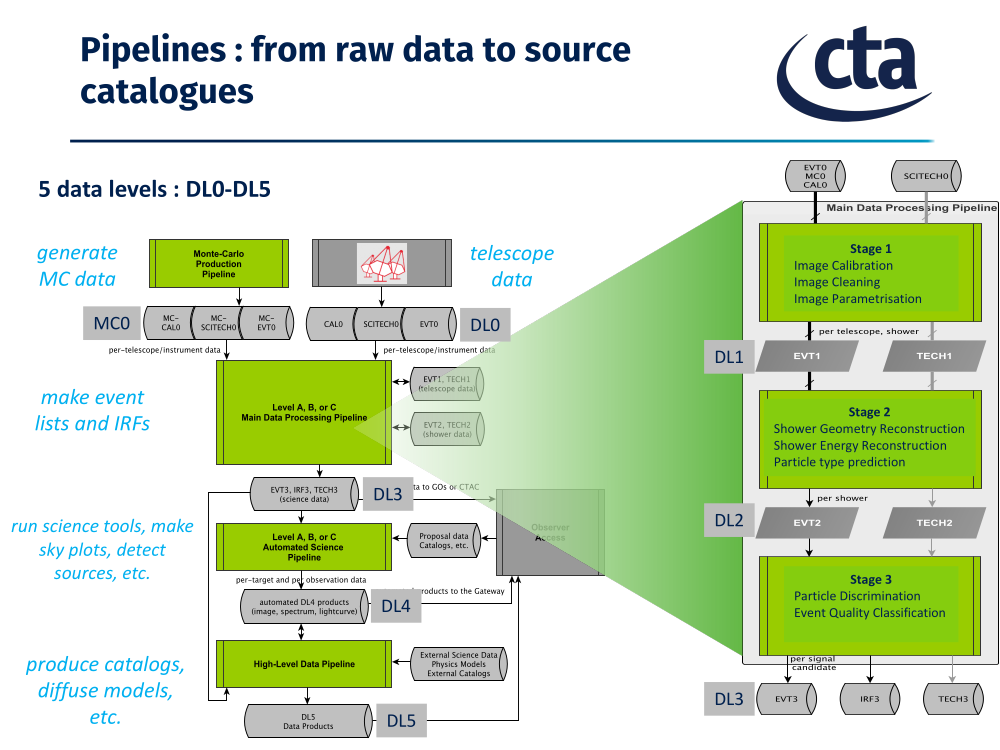
\includegraphics[width=\linewidth]{CTADataLevels.png}
	\caption[Flux des données CTAO]{Flux des données CTAO. Source: \cite{CTAOComputingChallenges}, page 5}
\end{figure}

\begin{itemize}
	\item MC0 : Données créées par des simulateurs Monte-Carlo
	\item DL0 : Données réelles récupérées par les télescopes
	\item DL1 : Images calibrées et nettoyées (par télescope/pluie Cherenkov)
	\item DL2 : Reconstruction de la pluie selon les images récupérées et prédiction de type hadronique/électromagnétique
	\item DL3 : Qualification et discrimination des pluies
	\item DL4 : Analyse des données de haut-niveau (spectres du ciel complet, etc.)
	\item DL5 : Agrégation des données pour en créer des catalogues et en tirer des conclusions scientifiques.
\end{itemize}

\subsection{Flux logiciel}

\begin{figure}[tbph!]
	\centering
	\includegraphics[width=\linewidth]{CTLearnWorkflow.png}
	\caption[Flux du logiciel CTLearn]{Flux du logiciel CTLearn. Source: \cite{CTLearnWorkflow}}
\end{figure}

Les données utilisées par CTLearn sont les signaux numérisés de chaque capteur composant la caméra d'un télescope, données de niveau DL1.
Ces données sont récupérées via les outils CTAPipe et DL1-Data-Handler. 
Ce projet de bachelor résiderait donc entre DL1-Data-Handler et CTLearn ou serait intégré à l'un d'entre eux comme étape de pré-traitement des signaux individuels.
% !TeX spellcheck = fr_FR
\chapter{Chapitre 3 : Méthodologie}

Dans ce projet, nous avons essayé de créer un programme capable d'analyser un signal temporel et 
d'en estimer la présence et la quantité de photons présent dans ce signal.

Pour cela, nous avons utilisé différents types de réseaux neuronaux qui sont eux-mêmes une technique de machine learning.
Ce chapitre se porte donc sur le fonctionnement des technologies et outils utilisés pour ce projet. 

\section{Machine learning}

Le machine learning peut être n'importe quel forme de programme ou système capable d'apprendre ou d'améliorer ses performances
en fonction des données qu'il traite.

Il existe deux types d'apprentissage pour le machine learning : supervisé et non supervisé.
Le premier signifie que les données utilisées pour entraîner un système contient aussi les conclusions qu'il doit en tirer.
Par exemple une image et un texte descriptif. Au fur et à mesure de l'analyse de ces différentes données, le système de machine learning
va trouver des informations ou motifs auxquels il va attribuer les conclusions prédéfinies.

Pour l'apprentissage non supervisé, le système de machine learning utilise des données brutes qui n'ont pas de conclusions ou descriptions associées.
Ce modèle va alors lui même essayer de trouver une manière de classifier ces données brutes ou de leur donner un score.

Dans le cadre de ce projet, l'équipe de l'\gls{unige} nous a fourni des données provenant de simulations des capteurs conçus pour les différents télescopes analysés.
Lors de la création de ces simulations, les méta-données des photons simulés ont aussi été sauvegardées, ce qui nous donne accès
à la "vérité" du moment exact ou chaque photon a été détecté, formalisant le corps du projet comme une recherche d'architecture de réseau neuronal avec un apprentissage supervisé.

\section{Réseaux neuronaux}

Alors, qu'est-ce qu'un réseau de neurones ou réseau neuronal exactement ?
Comme vu précédemment, c'est un modèle de machine learning qui est inspiré par le fonctionnement d'un cerveau humain.

Cette technique utilise des noeuds (neurones artificiels) interconnectés entre eux, créant des couches similaires à nos cerveaux.
Chaque noeud peut être ou non connecté à un ou plusieurs neurones supplémentaires permettant une infinité de configurations possibles.
La configuration d'un réseau de neurones est aussi surnommée l'architecture du réseau.

\subsection{Les perceptrons}

Chacun des noeuds qui composent un réseaux de neurones fonctionne comme une fonction mathématique, prenant des valeurs d'entrée et une valeur de sortie.
Ces neurones sont aussi appelés perceptrons et suivent en général le fonctionnement suivant :

\begin{figure}[tbph!]
	\centering
	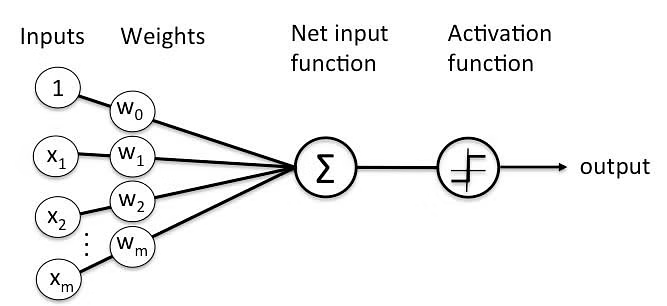
\includegraphics[width=0.6\linewidth]{perceptron.png}
	\caption[Illustration d'un perceptron]{Illustration d'un perceptron. Source : \cite{PerceptronImage}}
\end{figure}

Les paramètres d'un perceptron sont : un biais, et $x$ données d'entrées avec des poids associés. Toutes ces valeurs pondérées sont ensuite additionnées ensemble
et passées à une fonction d'activation qui donnera la valeur finale de sortie au perceptron. En général, la fonction d'activation est une sigmoïde, 
mais pourrait être n'importe quelle fonction mathématique qui s'adapterait mieux au problème que l'on essaye de résoudre.

Avec un seul perceptron, il est possible d'ajuster ces poids de manière à lui faire apprendre une motif de
séparation linéaire en fonction des données d'entrée. 

\begin{figure}[tbph!]
	\centering
	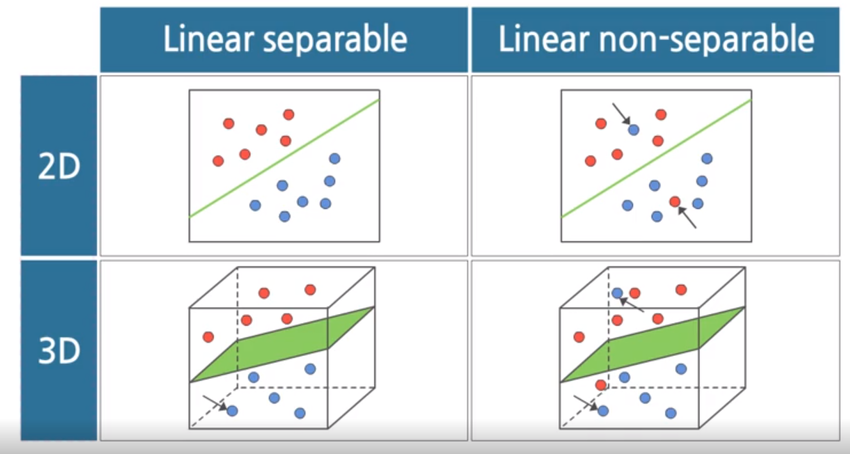
\includegraphics[width=0.4\linewidth]{separation-lineaire.png}
	\caption[Comparaison de données séparables ou non linéairement]{Comparaison de données séparables ou non linéairement. Source : \cite{LinearSeparation}}
\end{figure}

Il a donc été rapidement imaginé d'interconnecter ces perceptrons pour permettre d'apprendre des problèmes non linéaires. 
Créant l'architecture la plus simple le "Multi Layer Perceptron" ou perceptron multi-couches.

\subsection{Multi Layer Perceptron}

Cette architecture de réseaux de neurones consiste simplement à créer 3 types de couches avec un nombre variable de perceptrons pour chacune d'entre elles :

\begin{figure}[tbph!]
	\centering
	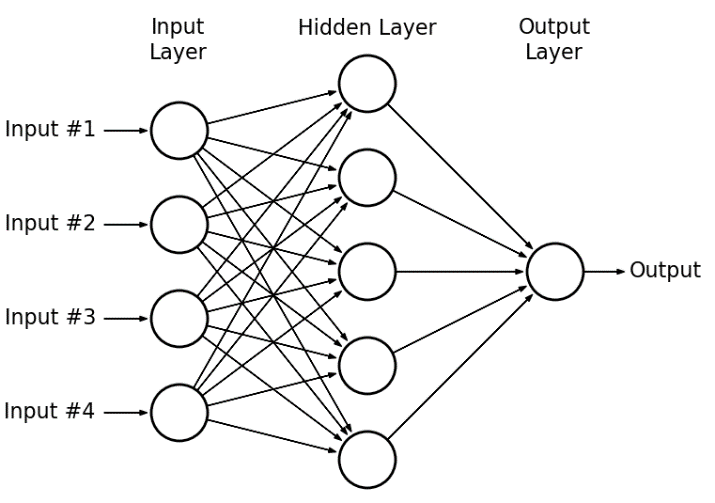
\includegraphics[width=0.4\linewidth]{MLP.png}
	\caption[Exemple d'un perceptron multi-couches]{Exemple d'un perceptron multi-couches. Source : \cite{MLPImage}}
\end{figure}

\begin{itemize}
	\item 1 couche d'entrée : Cette couche représente seulement les valeurs d'entrées de manière organisée, 
	par exemple une image de 10x10 pixels aurait une couche de taille 100. 
	\item $x$ nombre de couches cachées : Ici un nombre de couches indéterminées peuvent être ajoutées. 
	Chacune d'entre elles peuvent avoir un nombre de neurones différents dépendant du problème à traiter.
	\item 1 couche de sortie : Cette couche peut aussi avoir une taille variable dépendant de ce que le modèle doit accomplir. 
	Par exemple, si le modèle à comme but de détecter si une image est un chat ou non, cette couche pourrait n'avoir qu'un neurone avec une fonction d'activation sigmoïde.
\end{itemize}

Entre chacune de ces couches, chaque neurone est connecté avec chacun des autres de la couche suivante, créant des couches surnommées "denses".

\subsection{Apprentissage}

Peu importe le nombre de couches ou de neurones qui composent un réseau, il faut bien que celui-ci apprenne à résoudre le problème pour lequel il a été conçu.
Cet apprentissage se repose sur les bases mathématiques que le perceptron utilise. 
Lorsque l'on calcule le résultat d'un perceptron, celui-ci va calculer une ou plusieurs valeurs en sortie.
Lors d'un apprentissage supervisé, les valeurs de sortie attendues sont connues. On peut calculer une valeur d'erreur avec une fonction mathématique.
Nous avons donc volonté dans ce cas de minimiser cette fonction d'erreur. Et il est possible de le faire en modifiant les poids des valeurs d'entrées. 
La manière de trouver comment modifier ces poids s'appelle la descente de gradient.

\begin{figure}[tbph!]
	\centering
	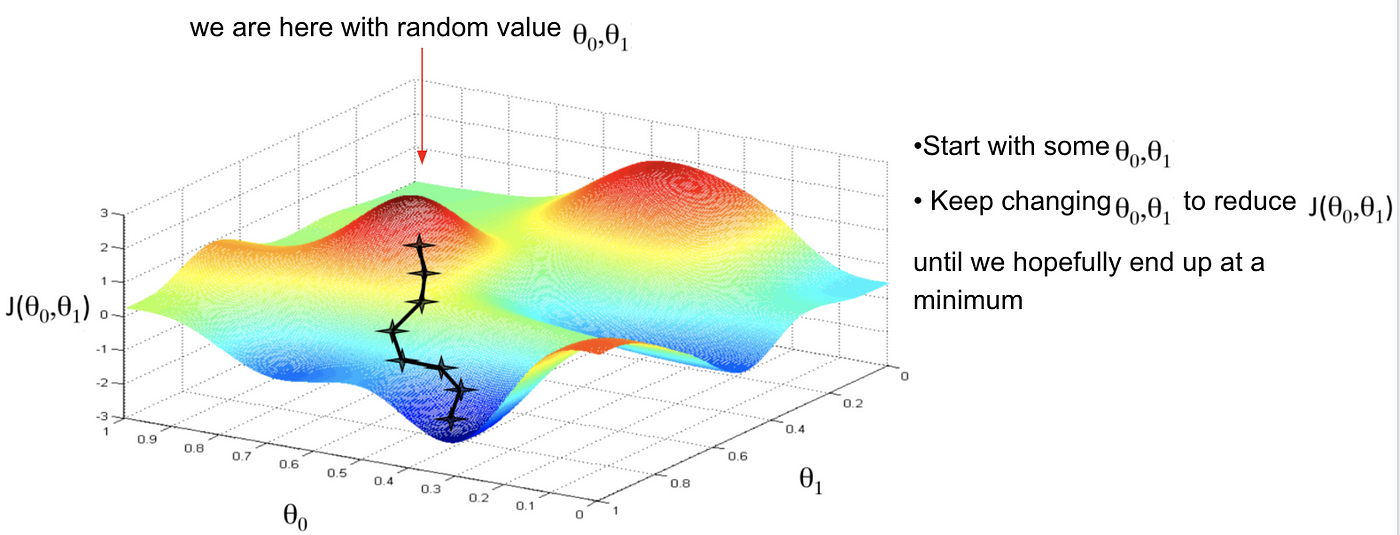
\includegraphics[width=0.8\linewidth]{gradient_descent.png}
	\caption[Exemple d'une descente de gradient en 3D]{Exemple d'une descente de gradient en 3D. Source : \cite{GradientDescentImage}}
\end{figure}

Il est possible de trouver comment modifier les valeurs de chaque poids ou biais
de chaque neurones afin de minimiser la fonction d'erreur et cela s'appelle la "backward propagation error" ou
"backpropagation".

Un piège fréquent lors de l'entraînement de réseaux neuronaux est l'overfitting. Le processus d'apprentissage fonctionne parfois trop "bien"
sur les données utilisées, jusqu'au point que le réseau de neurones y trouve des motifs qui ne sont pas ceux que l'on attend.

Par exemple, pour un réseau essayant de différencier des images de chaussures d'autres vêtements. 
Si, toutes les chaussures sont vertes dans les données d'entraînement, le réseau pourrait en déduire 
que c'est la couleur qui permet de les différencier. Cependant, lorsque le modèle se verra présenter
une chaussure rouge ne faisant pas partie des données d'entraînement, celui-ci ne la reconnaîtra pas 
à cause de son mauvais entraînement.

\subsection{Réseau de neurones convolutif}

Comme évoqué précédemment, il existe une infinité de configurations pour un réseau de neurones, alors nous ne regarderons que 
en détail les différentes configurations qui ont été envisagées dans ce projet.

L'une des premières architectures de réseau neuronal qui a été envisagée pour ce projet à été le réseau de neurones convolutif.
Celui-ci consiste à certaines couches cachées d'une manière spécifique qui effectuera le même calcul qu'une convolution.

\begin{figure}[tbph!]
	\centering
	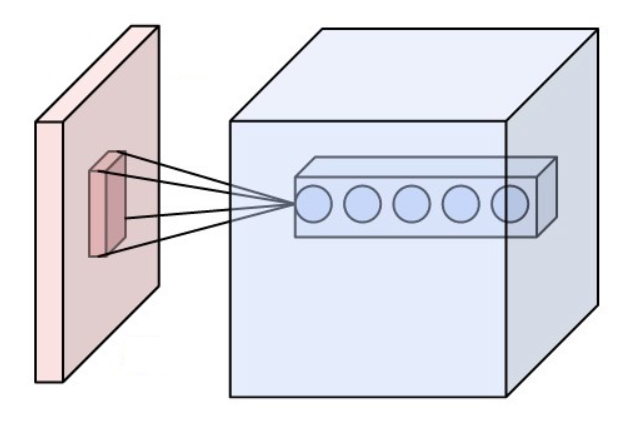
\includegraphics[width=0.4\linewidth]{Conv_layer.png}
	\caption[Illustration d'une couche convolutive de réseau neuronal]{Illustration d'une couche convolutive de réseau neuronal. Source : \cite{ConvImage}}
\end{figure}

L'opération de convolution en mathématique permet généralement d'extraire des informations d'une image comme le taux de 
variation d'intensité entre chaque pixel lors d'une détection de contours par exemple.
Ici, la différence est que le noyau utilisé pour la convolution n'est pas un noyau provenant d'algorithmes comme Sobel ou Canny mais ce sera
l'apprentissage du réseau qui va établir un noyau le plus optimisé pour trouver les caractéristiques recherchées dans les données d'entrée.

\subsection{Réseau de neurones récurrents}

Un autre type de réseau neuronal est le réseau de neurones récurrents. Cette architecture est adaptée
à des problèmes comprenant des données séquentielles ou temporelles généralement comme de la détection automatique de parole ou de texte.

Cette architecture diffère des autres réseaux de neurones car elle contient un mécanisme de "mémoire" intégré dans le modèle.
La mémoire est généralement implémentée en connectant la sortie de chaque neurone comme une entrée supplémentaire au prochain neurone de cette même couche.

\begin{figure}[tbph!]
	\centering
	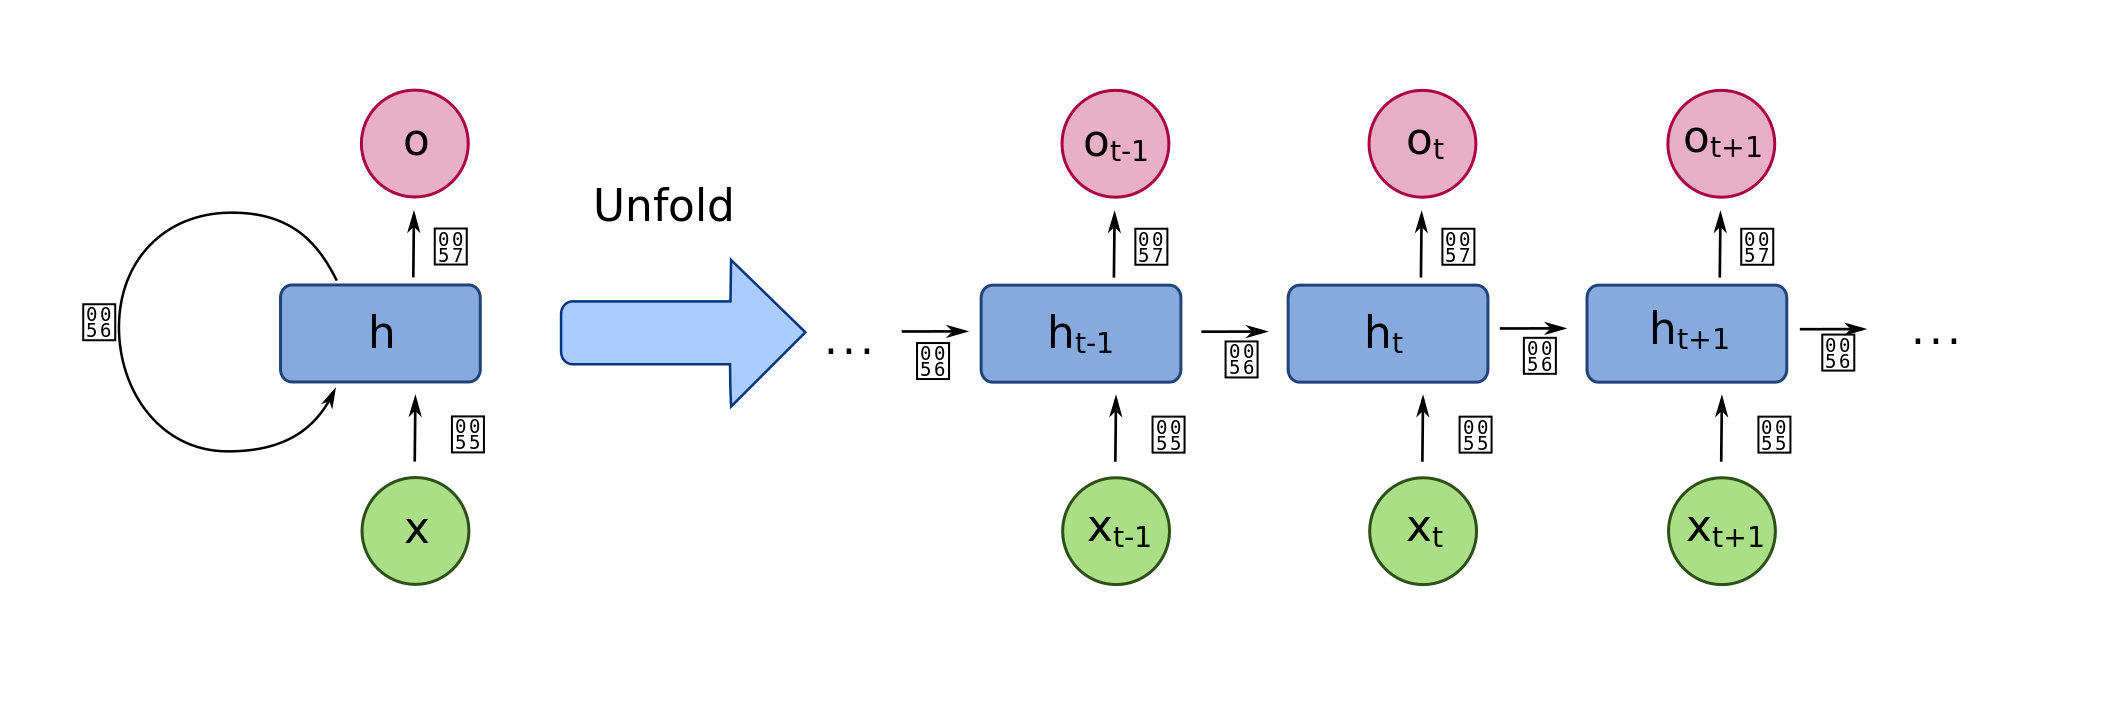
\includegraphics[width=0.8\linewidth]{rnn.png}
	\caption[Illustration de réseau de neurones récurrents]{Illustration de réseau de neurones récurrents. Source : \cite{RnnImage}}
\end{figure}

Cette "mémoire" n'existe que de manière temporaire à chaque exécution du réseau. Certaines autres configurations tel que les LSTM pour "Long and Short Term Memory"
sont aussi capables de mémoriser des informations à plus long terme.

\subsection{Auto-encodeurs}

Lors de la première partie de ce projet se focalisant sur les problématiques du télescope Terzina, un autre type de réseau 
avait été envisagé pour sa capacité à compresser des données : les auto-encodeurs.

L'auto-encodeur est une architecture de réseaux de neurones particulière qui comprend deux parties distinctes d'encodage et de décodage. 
Ces deux étapes peuvent aussi être perçues comme une compression et décompression successive. \cite{IbmAutoencoder}

\begin{figure}[tbph!]
	\centering
	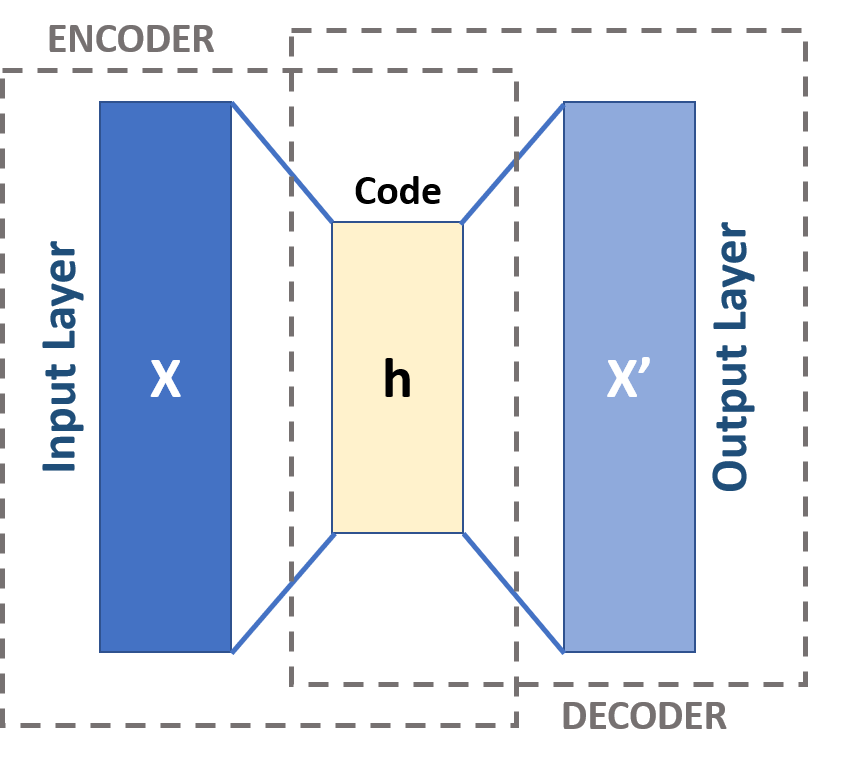
\includegraphics[width=0.4\linewidth]{Autoencoder.png}
	\caption[Schéma d'auto-encodeur]{Schéma d'auto-encodeur. Source : \cite{Autoencoder}}
\end{figure}

En entraînant le réseau de neurones, celui-ci va apprendre à réduire les informations en entrée jusqu'à un minimum pour 
ensuite essayer de reproduire au mieux les données originales à partir de cette représentation réduite.
Ceci résulte en général en une perte de précision des données lors de la compression.

\subsection{Couches}
Les configurations vues jusqu'à maintenant peuvent aussi être combinées entre elles pour former de plus grand réseaux de neurones.
Les réseaux neuronaux peuvent donc avoir une partie de réseau CNN et RNN, etc. Chacune des couche peut ainsi être catégorisée par
rapport à sont utilité.
Il existe aussi plus de couches spécifiques capables de travail spécifique. En voici plusieurs utilisées au cours de ce travail ainsi que leur utilité :

\subsubsection{BatchNormalisation}
La couche "BatchNormalisation", en général utilisée en premier dans un réseau, sert à normaliser les données qui lui sont données.
Cela sert à généraliser le reste du traitement du réseau, par exemple si l'on traitait des images avec des expositions différentes.

\subsubsection{Flatten}
Lors de l'utilisation de couches de convolution, il est possible d'en effectuer plusieurs en même temps et de les traiter parallèlement.
On peut ensuite utiliser une couche "Flatten" pour rassembler ces données en une seule dimension.

\subsubsection{Pooling}
Ce type de couches dans un réseau neuronal permet de réduire le nombre de dimensions qui lui sont données en entrée.
Ses utilités sont de réduire la quantité de calculs pour la suite du réseau et de diminuer l'overfitting lors de l'entraînement.

Les deux manières les plus communes pour effectuer un pooling est de garder la moyenne ou le maximum de chaque dimension :

\begin{figure}[tbph!]
	\centering
	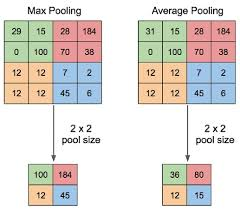
\includegraphics[width=0.4\linewidth]{pooling_layers.jpeg}
	\caption[Illustration du principe de Pooling]{Illustration du principe de Pooling. Source : \cite{PoolingImage}}
\end{figure}

\subsubsection{Dropout}
Cette couche a la même utilité que le Pooling, en réduisant le nombre d'entrées qui sont passés à la suite du réseau afin d'en diminuer l'overfitting.
Cependant, ici, seul un pourcentage des noeuds seront gardés au lieu de transformer les dimensions du réseau.

\section{Données}

Une autre grande partie de ce projet à été la gestion des données utilisées pour tester les différents réseaux de neurones.

\subsection{Pe Extractor}

Le premier simulateur qui a été fourni provenait d'un projet existant de l'\gls{unige} s'appelant "pe\_extractor".
Ce projet Python contient un générateur de signal avec du bruit NSB dans lequel des \gls{pe} sont insérés.
Le concept de photon-électron ou \gls{pe} est l'interaction physique lorsqu'un photon est détecté par un capteur et converti en charge électromagnétique analogique.
Cette quantité électromagnétique est appelée photon-électron.

Le bruit NSB pour un télescope est le bruit de fond minimum lorsqu'il pointe le ciel pendant la nuit. Même dans ces meilleures conditions,
de la lumière provenant des villes et de l'atmosphère est détectée par le télescope. 
De manière aléatoire et selon une fréquence donnée, le générateur ajoute au signal l'amplitude simulée d'un photon-électron.
Cette amplitude est définie par un fichier d'impulsion qui dépend du capteur utilisé.

Le générateur fournit deux tableaux en sortie : le signal discrétisé et des bacs contenant la vérité du nombre de \gls{pe} ayant été injectés sur cette période.

Voici les paramètres importants du générateur et leur explication :
\begin{enumerate}
    \item "pe\_rate\_mhz" : Définit la fréquence moyenne à laquelle un \gls{pe} est injecté dans le signal.
        L'injection de \gls{pe} est aléatoire en suivant une distribution Poisson.
    \item "sampling\_rate\_mhz" : Définit la vitesse d'échantillonnage du signal. Pour Terzina, elle est de 200MHz.
    \item "n\_sample" et "n\_sample\_init" : Le générateur a un mécanisme d'initialisation pour le bruit électrique 
        qui peut prendre un certain nombre de cycles pour commencer a créer des informations cohérentes au niveau physique, 
        ces deux paramètres peuvent donc contrôler un nombre d'échantillons à écarter au début de la génération.
    \item "bin\_size\_ns" : Ce paramètre gère la période de comptabilisation des \gls{pe} insérés dans le signal de sortie.
    \item "shift\_proba\_bin" : Permet de décaler la comptabilisation de l'insertion de signal par un certain nombre de bacs.
        Ce système existe car l'impulsion a un temps de montée avant d'atteindre son pic, ce qui permet de décaler les bacs 
        de vérité pour s'aligner avec le pic de l'impulsion.
    \item "sigma\_smooth\_pe\_ns" : Ce paramètre sert à répartir le compte des \gls{pe} insérés sur les bacs voisins en ns
        pour éviter une vérité entière. 
    \item "noise\_lsb" : Est une quantité de bruit électronique.
\end{enumerate}

Normalement, les paramètres sont tels que, le nombre de bacs simulés est plus grand que le nombre d'échantillons générés pour le signal.
Une première adaptation a été programmée pour regrouper ces bacs sur la même fréquence d'échantillonnage du signal :

\begin{figure}[tbph!]
	\centering
	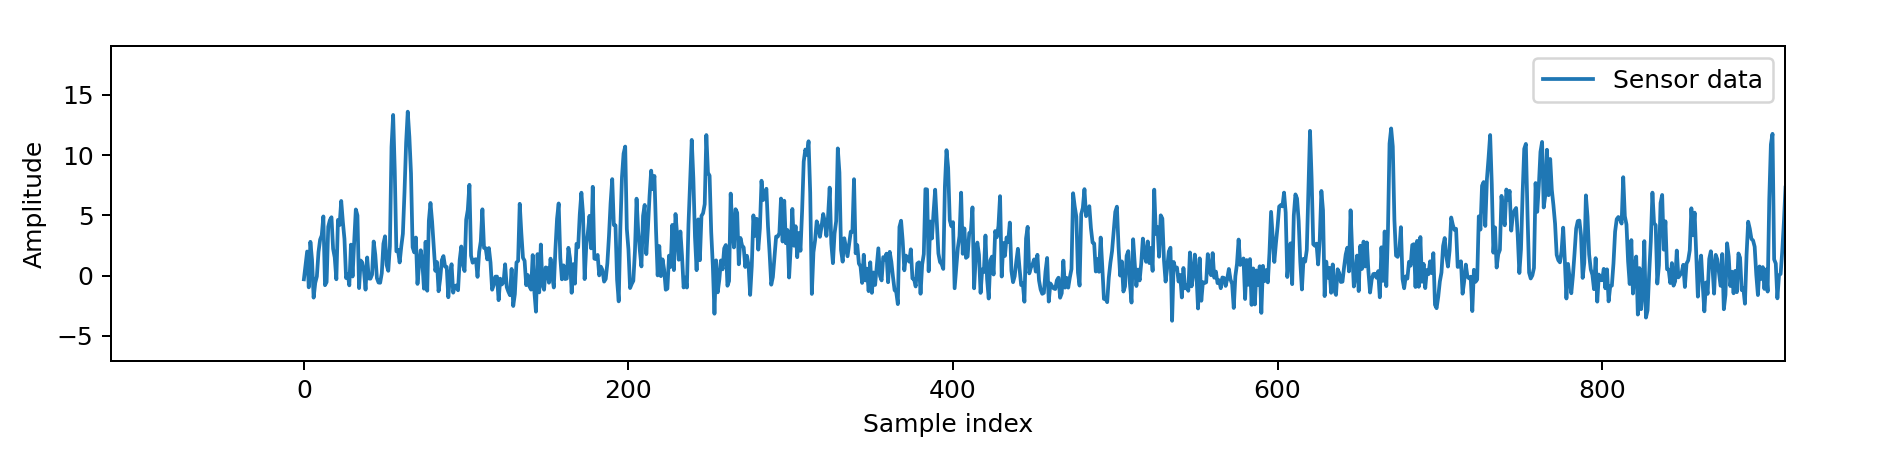
\includegraphics[width=\linewidth]{sensor_waveform.png}
	\caption[Exemple de signal simulé]{Exemple de signal simulé.}
\end{figure}

\subsection{Fichiers de simulation Corsika}

Le premier simulateur de signal provenant de "pe\_extractor" ne simule que des interférences de type NSB. 
Pour se rapprocher des données réelles des caméras, il a été choisi de récupérer des fichiers de simulation de pluies Cherenkov pour le \gls{lst}.

Ces fichiers de simulations contiennent énormément de données, de la configuration du télescope jusqu'à l'impact des photons provenant des pluies Cherenkov.
Ceux-ci sont stockés sur le partage de fichiers du cluster Yggdrasil de l'\gls{unige} sous un format de fichier ROOT. 

ROOT est un framework logiciel conçu par le \gls{cern} pour l'analyse de données et la gestion d'entrées et sorties. Ces types de fichiers
sont souvent utilisés pour stocker de manière structurée des données provenant d'expériences scientifiques en tant qu'arbres et tableaux
pour réduire l'espace de stockage utilisé par un ficher.

Ces différentes données ne sont pas utilisables directement et doivent être réinterprétées par le logiciel "pyeventio\_example", lui aussi fourni
par l'équipe de l'\gls{unige}. Ce projet met à disposition un exécutable nommé "runana". Celui-ci permet de créer un fichier binaire 
contenant des métadonnées, le signal de chaque capteur composant la caméra du télescope et les instants auxquels les photons 
provenant de la pluie Cherenkov ont impacté les capteurs.

% \section{Outils}
% \subsection{Tensorflow}
% \subsection{Tensorboard}
% \subsection{Keras}
% \subsection{Jupyter notebook}
% \subsection{IPython notebook}
% !TeX spellcheck = fr_FR
\chapter{Chapitre 4 : Résultats}

%TODO comparaisons qui soient bien justifiées et qui soient dans le même pipeline et données

%TODO Faire un chapitre sur la gestion des données et complexité de cela

\section{Prototypage}
Pour débuter le prototypage, j'ai commencé à mettre en place un réseau neuronal convolutif de régression simple qui prend en 
entrée une fenêtre de taille fixe, qui contiendra les échantillons du signal de manière séquentielle dans le temps.
Et dont le résultat est une estimation de la probabilité qu'un \gls{pe} soit présent au centre de la fenêtre analysée :

\begin{figure}[tbph!]
	\centering
	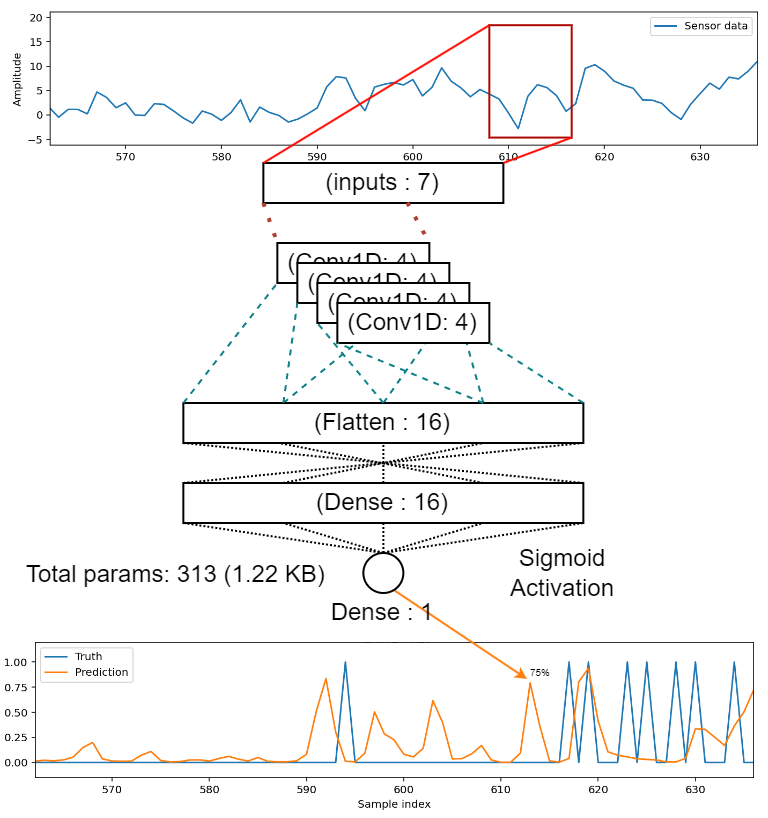
\includegraphics[width=0.6\linewidth]{cnn_simple.drawio.png}
	\caption[Diagramme de fonctionnement du premier CNN simple]{Diagramme de fonctionnement du premier CNN simple.}
\end{figure}

Le fonctionnement de cette architecture n'a pas donné de bons résultats, ceci à cause de plusieurs facteurs. Le premier est qu'à cause des paramètres
de bacs du générateur, les premiers tests effectués se basaient sur des données erronées car les impulsions n'étaient pas centrées au centre de la fenêtre.

Cette première expérience m'a aussi poussé à développer une vue au "cas par cas" où chaque inférence du modèle peut être examinée.
Cette vue affiche les données d'entrée, la vérité attendue et le résultat du modèle ce qui permet de confirmer les données d'entraînement de celui-ci. 

Cependant, même après avoir corrigé la configuration du générateur, les résultats, bien que légèrement améliorés, restaient non fiables à cause de beaucoup de
faux positif et faux négatifs.

Pour palier à cela, au lieu d'entraîner le modèle sur une seule vérité au centre de la fenêtre analysée, ce serait sur chaque 
échantillon que le réseau neuronal donnera une estimation de la présence ou non d'un \gls{pe}.

Ce nouveau modèle a immédiatement mieux performé que le précédant :

\begin{figure}[tbph!]
	\centering
	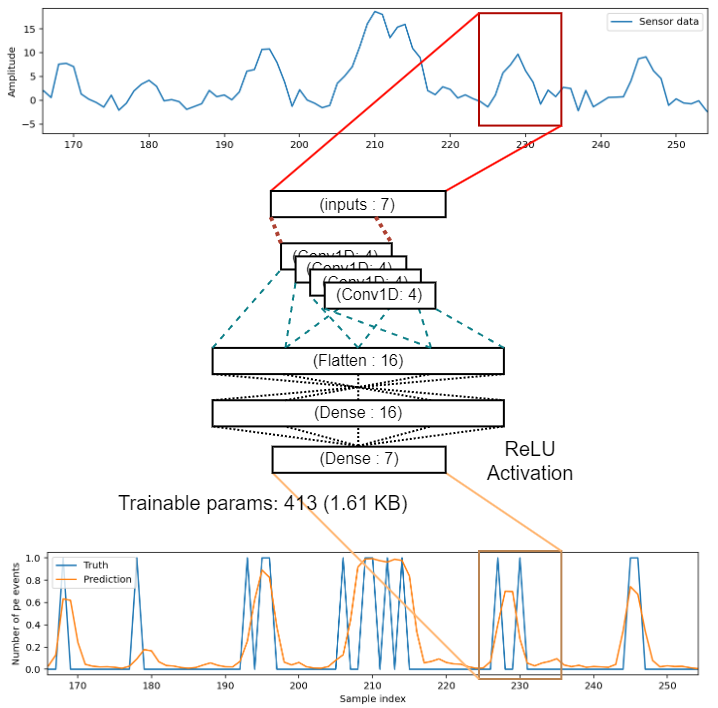
\includegraphics[width=0.6\linewidth]{cnn_mult.drawio.png}
	\caption[Diagramme de fonctionnement du deuxième CNN à multiple sortie]{Diagramme de fonctionnement du deuxième CNN à multiple sortie.}
\end{figure}

En modifiant les différents paramètres de chaque couche, il est aussi possible d'améliorer les performances de celui-ci.
De plus, en ne calculant plus la présence de manière booléenne mais en estimant la quantité de \gls{pe} présents 
en changeant la fonction d'activation finale pour utiliser la fonction mathématique "ReLU" qui n'est pas confinée 
à l'intervalle $ \left[ 0, 1\right] $ comme la sigmoïde mais à $ \left[0, +\infty\right[ $, il est possible d'entraîner le modèle
pour qu'il estime le nombre de \gls{pe} à un instant $t$ dans une fenêtre. 
% !TeX spellcheck = fr_FR
\chapter*{Conclusion}

\addcontentsline{toc}{chapter}{Conclusion} % Adding toc entry

Étant passionné par l'astronautique et intéressé par tous les sujets adjacents tels que l'astrophysique ou même l'aéronautique, 
j'ai été ravi d'être choisi pour participer à un projet concret touchant à ces mêmes domaines.

Pour rappel, l'objectif de ce projet de bachelor consistait à trouver un modèle de réseau neuronal capable d'interpréter 
le contenu de signaux produits par des télescopes afin d'identifier les possibles photons provenant de pluies atmosphériques Cherenkov.
Le modèle trouvé aurait servi à deux usages : le premier à réduire le stockage et le traitement des données en participant 
au tri d'événements scientifiquement intéressants, le deuxième à possiblement améliorer les performances d'analyse de plus haut niveau 
en filtrant le bruit contenu dans les signaux. 

Pour réaliser ce projet, j'ai d'abord dû appréhender le phénomène physique de la radiation Cherenkov et ses implications pour le domaine de l'astrophysique.
Il m'a fallu aussi comprendre le fonctionnement des différents télescopes existants et futurs afin de discerner 
ce qui était attendu de ce projet. J'y ai appliqué les bases en machine learning que j'ai appris lors de mon cursus, et ai 
réussi à éviter plusieurs pièges du domaine. J'ai aussi dû prendre en main plusieurs outils simulant des données scientifiques et les adapter
pour entraîner des modèles de machine learning. Malgré les diverses techniques de machine learning testées,
aucun des modèles n'a présenté des performances permettant à celui-ci d'être intégré au sein d'autres projets comme imaginé.

Cependant, la détection de \gls{pe} d'un signal n'est pas encore a considérer comme impossible. 
Il reste encore des techniques de machine learning plus complexes a investiguer. 
De plus et comme évoqué au chapitre précédent, si mon soupçon que les données ne contiennent pas assez de détails s'avérait exact, il est envisageable d'observer
les données d'une manière différente pour minimiser les effets de bruits. Par exemple, en observant des groupes de pixels voisins. 
Il se pourrait aussi qu'il est impossible de discerner la présence de petites quantités de \gls{pe} dans des pluies de très basse énergie.

Dans l'ensemble, je suis satisfait du travail que j'ai pû fournir au cours de ces derniers mois.
Grâce à cette expérience, j'ai pu améliorer mes connaissances en machine learning et en recherches scientifiques.
Dans un monde se tournant de plus en plus vers les intelligences artificielles et le machine learning,
il est certain que les apprentissages et les conclusions que j'ai acquis au cours de ce travail me seront d'une 
grande utilité durant toute ma carrière professionnelle.
% % !TeX spellcheck = fr_FR
% \addcontentsline{toc}{chapter}{Annexes} % Adding toc entry
% %%% COMMENT THESES LINES IF YOU DO NOT USE DEDICATED TOC FOR ANNEXES
% \stopcontents[default]
% \resumecontents[annexes]
% %%% /COMMENT THESES LINES IF YOU DO NOT USE DEDICATED TOC FOR ANNEXES
% \chapter*{Annexes}

% % \begin{center}
% % \textit{Imprimer idéalement cette page sur une page de couleur.}
% % \textit{Chaque annexe doit commencer sur une nouvelle page et doit être numérotée : Annexe 1 puis Annexe 2, etc.}
% % \end{center}


% \chapter*{Annexe 1}
% \addcontentsline{toc}{chapter}{Annexe 1}


% \chapter*{Annexe 2}
% \addcontentsline{toc}{chapter}{Annexe 2}


% \chapter*{Annexe 3}
% \addcontentsline{toc}{chapter}{Annexe 3}


% %%% COMMENT THESES LINES IF YOU DO NOT USE DEDICATED TOC FOR ANNEXES
% \stopcontents[annexes]
% \resumecontents[default]
% %%% /COMMENT THESES LINES IF YOU DO NOT USE DEDICATED TOC FOR ANNEXES
% !TeX spellcheck = fr_FR
% \chapter*{Bibliographie}

% \noindent\textit{Sites Web consultés – Code repris d’ailleurs – Notices techniques – Articles de presse – Ouvrage imprimés – Ouvrages électroniques – Chapitre dans un ouvrage imprimé – Rapports imprimés – Travaux universitaires – Articles de revues imprimés – Articles de périodiques électroniques – Communication dans un congrès. Pour chacun de ces types de document, les mise en forme sont dans le document « Méthode de citation et de rédaction d’une bibliographie ».}\\

% \textit{Afin de gagner du temps, pensez à utiliser le logiciel de gestion bibliographique Zotero (et/ou BibTeX si vous utilisez LaTeX) pour la mise en forme et l’édition automatique de vos références à la norme ISO690.}
\nocite{*}
\addcontentsline{toc}{chapter}{Bibliographie} % Adding toc entry
\printbibliography
\end{spacing}
\end{document}
%%%%%%%%%%%%%%%%%%%%%%%%%%%%%%%%%% DOCUMENT ENDS HERE %%%%%%%%%%%%%%%%%%%%%%%%%%
